\documentclass[12pt,twocolumn,tighten]{aastex62}
%\pdfoutput=1 %for arXiv submission
\usepackage{amsmath,amstext,amssymb}
\usepackage[T1]{fontenc}
\usepackage{apjfonts}
\usepackage[figure,figure*]{hypcap}
\usepackage{graphics,graphicx}
\usepackage{hyperref}
\usepackage{comment}
\usepackage{todonotes}

\renewcommand*{\sectionautorefname}{Section} %for \autoref
\renewcommand*{\subsectionautorefname}{Section} %for \autoref

%% Reintroduced the \received and \accepted commands from AASTeX v5.2.
%% Add "Submitted to " argument.
\received{\today}
\revised{---}
\accepted{---}
\submitjournal{AAS journals.}

\shortauthors{Bouma et al.}
\shorttitle{Early Arrival of WASP-4\lowercase{b}}

\NewPageAfterKeywords

\begin{document}

\title{WASP-4\lowercase{b} Arrived Early for the TESS Mission}

\correspondingauthor{L. G. Bouma}
\email{luke@astro.princeton.edu}

\author[0000-0002-0514-5538]{L. G. Bouma}
\affiliation{ Department of Astrophysical Sciences, Princeton
University, 4 Ivy Lane, Princeton, NJ 08540, USA}
%
\author[0000-0002-4265-047X]{J. N. Winn}
\affiliation{ Department of Astrophysical Sciences, Princeton
University, 4 Ivy Lane, Princeton, NJ 08540, USA}
%
\author[0000-0002-0875-8401]{J.-M. D\'esert}
\affiliation{ API, University of Amsterdam, P.O. Box 94249, 1090 GE
Amsterdam, The Netherlands}
%
\author[0000-0002-3481-9052]{K. G. Stassun}
\affiliation{Vanderbilt University, Department of Physics \& Astronomy,
6301 Stevenson Center Lane, Nashville, TN 37235, USA}
\affiliation{Fisk University, Department of Physics, 1000 17th Avenue
N., Nashville, TN 37208, USA}
%
\author[0000-0002-6939-9211]{T. Daylan}
\affiliation{ Department of Physics and Kavli Institute for Astrophysics
and Space Research, Massachusetts Institute of Technology, Cambridge, MA
02139, USA }
%
\author[0000-0002-7084-0529]{S. Kane}
\affiliation{Department of Earth Sciences, University of California,
Riverside, CA 92521, USA}
% 
%-------------------------------------
% TESS Mission Architects:
% These authors should be listed in this order
% see https://spacebook.mit.edu/pages/viewpage.action?pageId=24543276
%-------------------------------------
%
\author{G. R. Ricker} % grr@space.mit.edu WAITING
\affiliation{ Department of Physics and Kavli Institute for Astrophysics
and Space Research, Massachusetts Institute of Technology, Cambridge, MA
02139, USA }
%
\author[0000-0001-6763-6562]{R. Vanderspek} % roland@space.mit.edu WAITING
\affiliation{ Department of Physics and Kavli Institute for Astrophysics
and Space Research, Massachusetts Institute of Technology, Cambridge, MA
02139, USA }
%
\author[0000-0001-9911-7388]{D. W.~Latham} % dlatham@cfa.harvard.edu WAITING
\affiliation{ Harvard-Smithsonian Center for Astrophysics, 60 Garden
Street, Cambridge, MA 02138, USA }
%
\author{S. Seager} % seager@mit.edu WAITING
\affiliation{ Department of Earth, Atmospheric, and Planetary Sciences,
Massachusetts Institute of Technology, Cambridge, MA 02139, USA }
%
\author[0000-0002-4715-9460]{J. M.~Jenkins} % jon.jenkins@nasa.gov WAITING
\affiliation{ NASA Ames Research Center, Moffett Field, CA 94035, USA }
%
%-------------------------------------
% 3 representatives of each of SPOC, POC, TSO, for a total of 9. 
%These 9 authors should be listed in alphabetical order
%-------------------------------------
% 3 TSO COAUTHORS
%
\author[0000-0002-3321-4924]{Z. Berta-Thompson} % Zachory.BertaThompson@Colorado.EDU WAITING
\affiliation{Department of Astrophysical and Planetary Sciences,
University of Colorado, Boulder, CO 80309, USA}
%
\author[0000-0001-8812-0565]{J. Rodriguez} % rodriguez.jr.joey@gmail.com WAITING
\affiliation{Harvard-Smithsonian Center for Astrophysics, 60 Garden
Street, Cambridge, MA 02138, USA }
%
\author[0000-0001-8020-7121]{K. Col\'on} % knicole.colon@nasa.gov WAITING
\affiliation{NASA Goddard Space Flight Center, Exoplanets and Stellar
Astrophysics Laboratory (Code 667), Greenbelt, MD 20771, USA}
% 3 SPOC COAUTHORS
%
\author[0000-0002-6778-7552]{J. D. Twicken} % Joseph.Twicken@nasa.gov WAITING
\affiliation{ NASA Ames Research Center, Moffett Field, CA 94035, USA }
\affiliation{ SETI Institute, Mountain View, CA 94043, USA}
%
\author{B. Wohler} % bill.wohler@nasa.gov WAITING
\affiliation{ NASA Ames Research Center, Moffett Field, CA 94035, USA }
\affiliation{ SETI Institute, Mountain View, CA 94043, USA}
%
\author[0000-0003-1963-9616]{D. A. Caldwell} % douglas.Caldwell@nasa.gov % WAITING
\affiliation{ NASA Ames Research Center, Moffett Field, CA 94035, USA }
\affiliation{ SETI Institute, Mountain View, CA 94043, USA}
%
%\\ \textcolor{red}{3 POC coauthors:}
\author{POC1}
\author{POC2}
\author{POC3}


\begin{abstract}
  %TODO: final numbers
  By combining data from the Transiting Exoplanet Survey Satellite (TESS)
  with data from previous studies, we show that the transit times of WASP-4b are
  incompatible with a constant orbital period.  The
  transits observed by TESS occurred $77.8 \pm 10.8$~seconds earlier than one would expect, based on the previous data.
  The orbital period appears to be shrinking by $\dot{P}=-12.1 \pm 1.2$
  milliseconds per year.   A simple clock offset is unlikely, because TESS observations of other
  hot Jupiter (WASP-6b, 18b, and 46b) are compatible with a constant period and rule out
  a 77.8-second offset at the 6.3$\sigma$ level.
  The timing variations seem to be astrophysical,
  and could be caused by apsidal precession, or perhaps by tidal
  decay.  The latter seems implausible on theoretical grounds, as it
  would require a stellar quality factor $Q_\star' \approx
  3\times10^4$.  Apsidal precession would imply an eccentricity
  $e\approx1.6\times 10^{-3}$, and the possibility of measuring the
  planet's Love number.  A Doppler shift from WASP-4's acceleration
  towards us could account for at most one quarter of the observed
  period change (at $2\sigma$).  Further observations will help
  confirm the reality of the timing variation, and eventually
  determine its cause.
\end{abstract}

\keywords{
  planet-star interactions ---
  planets and satellites: individual (WASP-4b, WASP-5b, WASP-6b,
    WASP-12b, WASP-18b, WASP-46b) ---
  binaries: close
}

\section{Introduction}
\label{sec:intro}

Long-term monitoring of hot Jupiter transit and occultation times
should eventually reveal two distinct processes.  First, whenever the
summed spin and orbital angular momenta in a hot Jupiter system fall
below a critical value, the system becomes unstable to tidal decay
\citep{counselman_outcomes_1973,hut_stability_1980}.  Most hot
Jupiters satisfy this condition; their orbits should be shrinking
\citep{levrard_falling_2009,matsumura_tidal_2010}.  The rate of decay
is uncertain, and depends on how friction dissipates energy carried by
gravitational tides (\citealt{ogilvie_tidal_2014} gives a review).  If
we could directly measure orbital decay rates, it would inform our
understanding of tidal dissipation.  This is important because the
dissipation rates determine the fate of the system.  During its
inspiral, if the planet fills its Roche lobe below the stellar
surface, the drag force from the stellar envelope accelerates the
inspiral, leading to a `direct-impact' merger
\citep{metzger_optical_2012,macleod_planetary_2018} Alternatively, if
the planet fills its Roche lobe above above the stellar surface, then
it could either be disrupted into an accretion disk or it could slowly
transfer mass to the star
\citep{metzger_optical_2012,valsecchi_tidally-driven_2015,jackson_tidal_2016}.
Further afield, the outcome of the eventual interaction between the
Earth and red giant Sun also hinges on the efficiency of tidal
dissipation \citep{rasio_tidal_1996}.

The second process that long-term timing studies should reveal is
rotation of the orbital ellipse within the orbital plane (apsidal
precession).  This effect has been studied extensively in eclipsing
binaries \citep[{\it e.g.},][]{
  schwarzschild_structure_1958,torres_accurate_2010,borkovits_eclipse_2015},
and has been explored theoretically for transiting planets
\citep{heyl_using_2007,pal_periastron_2008,jordan_observability_2008,ragozzine_probing_2009}.
However, apsidal precession has yet to be directly observed in hot
Jupiters, and the orbits would need non-zero eccentricity for it to be
detectable.  Though the eccentricities of hot Jupiters are expected to
be small, there are many mechanisms that could pump them away from
circularity (see \S~\ref{sec:apsidal_precession}, and
\citealt{bailey_understanding_2019}).  For hot Jupiters, the apsidal
precession is usually dominated by the quadrupolar distortion of the
planet by the star's tidal force \citep{ragozzine_probing_2009}.  The
observed precession rate in a hot Jupiter system can thus be used to
compute the planet's Love number, giving a third parameter along with
the mass and radius with which to describe the planet's interior
structure \citep[{\it e.g.},][who performed a similar procedure for
HAT-P-13b]{batygin_determination_2009}.  Measuring small
eccentricities and understanding their origin might also help us
understand the dynamical histories and inflated radii of hot Jupiters.
\citep[{\it
e.g.},][respectively]{dawson_origins_2018,ibgui_tidal_2010}

While numerous indirect studies have called attention to
population-level effects of tidal decay
\citep{jackson_observational_2009,hansen_calibration_2010,penev_constraining_2012,husnoo_observational_2012,matsakos_origin_2016,cameron_hierarchical_2018,penev_empirical_2018},
the most convincing direct evidence to date for either orbital decay
or apsidal precession has come from WASP-12b.
\citet{maciejewski_departure_2016} showed that the transit times of
WASP-12b did not follow a linear ephemeris at $5\sigma$ confidence,
and measured $\dot{P} = -26 \pm 4\,{\rm ms}\,{\rm yr}^{-1}$.  Using
new timing data, \citet{patra_2017} found $\dot{P} = -29 \pm 3\,{\rm
ms}\,{\rm yr}^{-1}$.  If the period change were caused entirely by
tidal decay, the implied modified stellar quality factor would be
$Q_\star' \approx 2\times10^5$.  Standard equilibrium tides do not
predict this level of dissipation
\citep{penev_tidal_2011,ogilvie_tidal_2014}.  The needed level of
friction might come from dynamical tides, or obliquity tides
\citep{weinberg_tidal_2017,millholland_obliquity_2018}.  The former is
more likely if WASP-12 is a subgiant, but the observational
constraints favor a main-sequence model
\citep{bailey_understanding_2019}.  More data are needed to understand
the WASP-12b timing variations.

This work focuses on the hot Jupiter WASP-4b, which orbits its host
star every 1.34 days, at a distance of $a/R_\star = 5.46$
\citep{wilson_wasp-4b_2008,hoyer_tramos_2013}.  WASP-4b is a plausible
candidate for orbital decay, in part because it has been frequently
observed over the past decade.  The host is a G7V dwarf, and is on the
main sequence (\S~\ref{sec:system_parameters}).  The orbit is
consistent with being circular (but see
\S~\ref{sec:apsidal_precession}), and having sky-projected obliquity
of zero
\citep{triaud_spin-orbit_2010,beerer_secondary_2011,sanchis-ojeda_starspots_2011}.

We measure new transit times for WASP-4b using TESS lightcurves
(\S~\ref{sec:observations},~\ref{sec:measurement}), and calculate the
system's parameters empirically (\S~\ref{sec:system_parameters}).  We
merge the new times with previous observations and compare three
models (\S~\ref{sec:timing}): a constant period, a decaying period,
and a slightly eccentric orbit undergoing precession.  We rule out a
constant period, but cannot firmly distinguish between the latter two
possibilities.  Each would have interesting implications
(\S~\ref{sec:implications}).  We rule out the possibility that a
systematic time system offset causes the observed variation
(Appendix~\ref{sec:verify_tess}), and conclude by advocating for
further monitoring of the system (\S~\ref{sec:future}).



\section{New transits and system parameters}
\begin{figure}[t]
    \begin{center}
        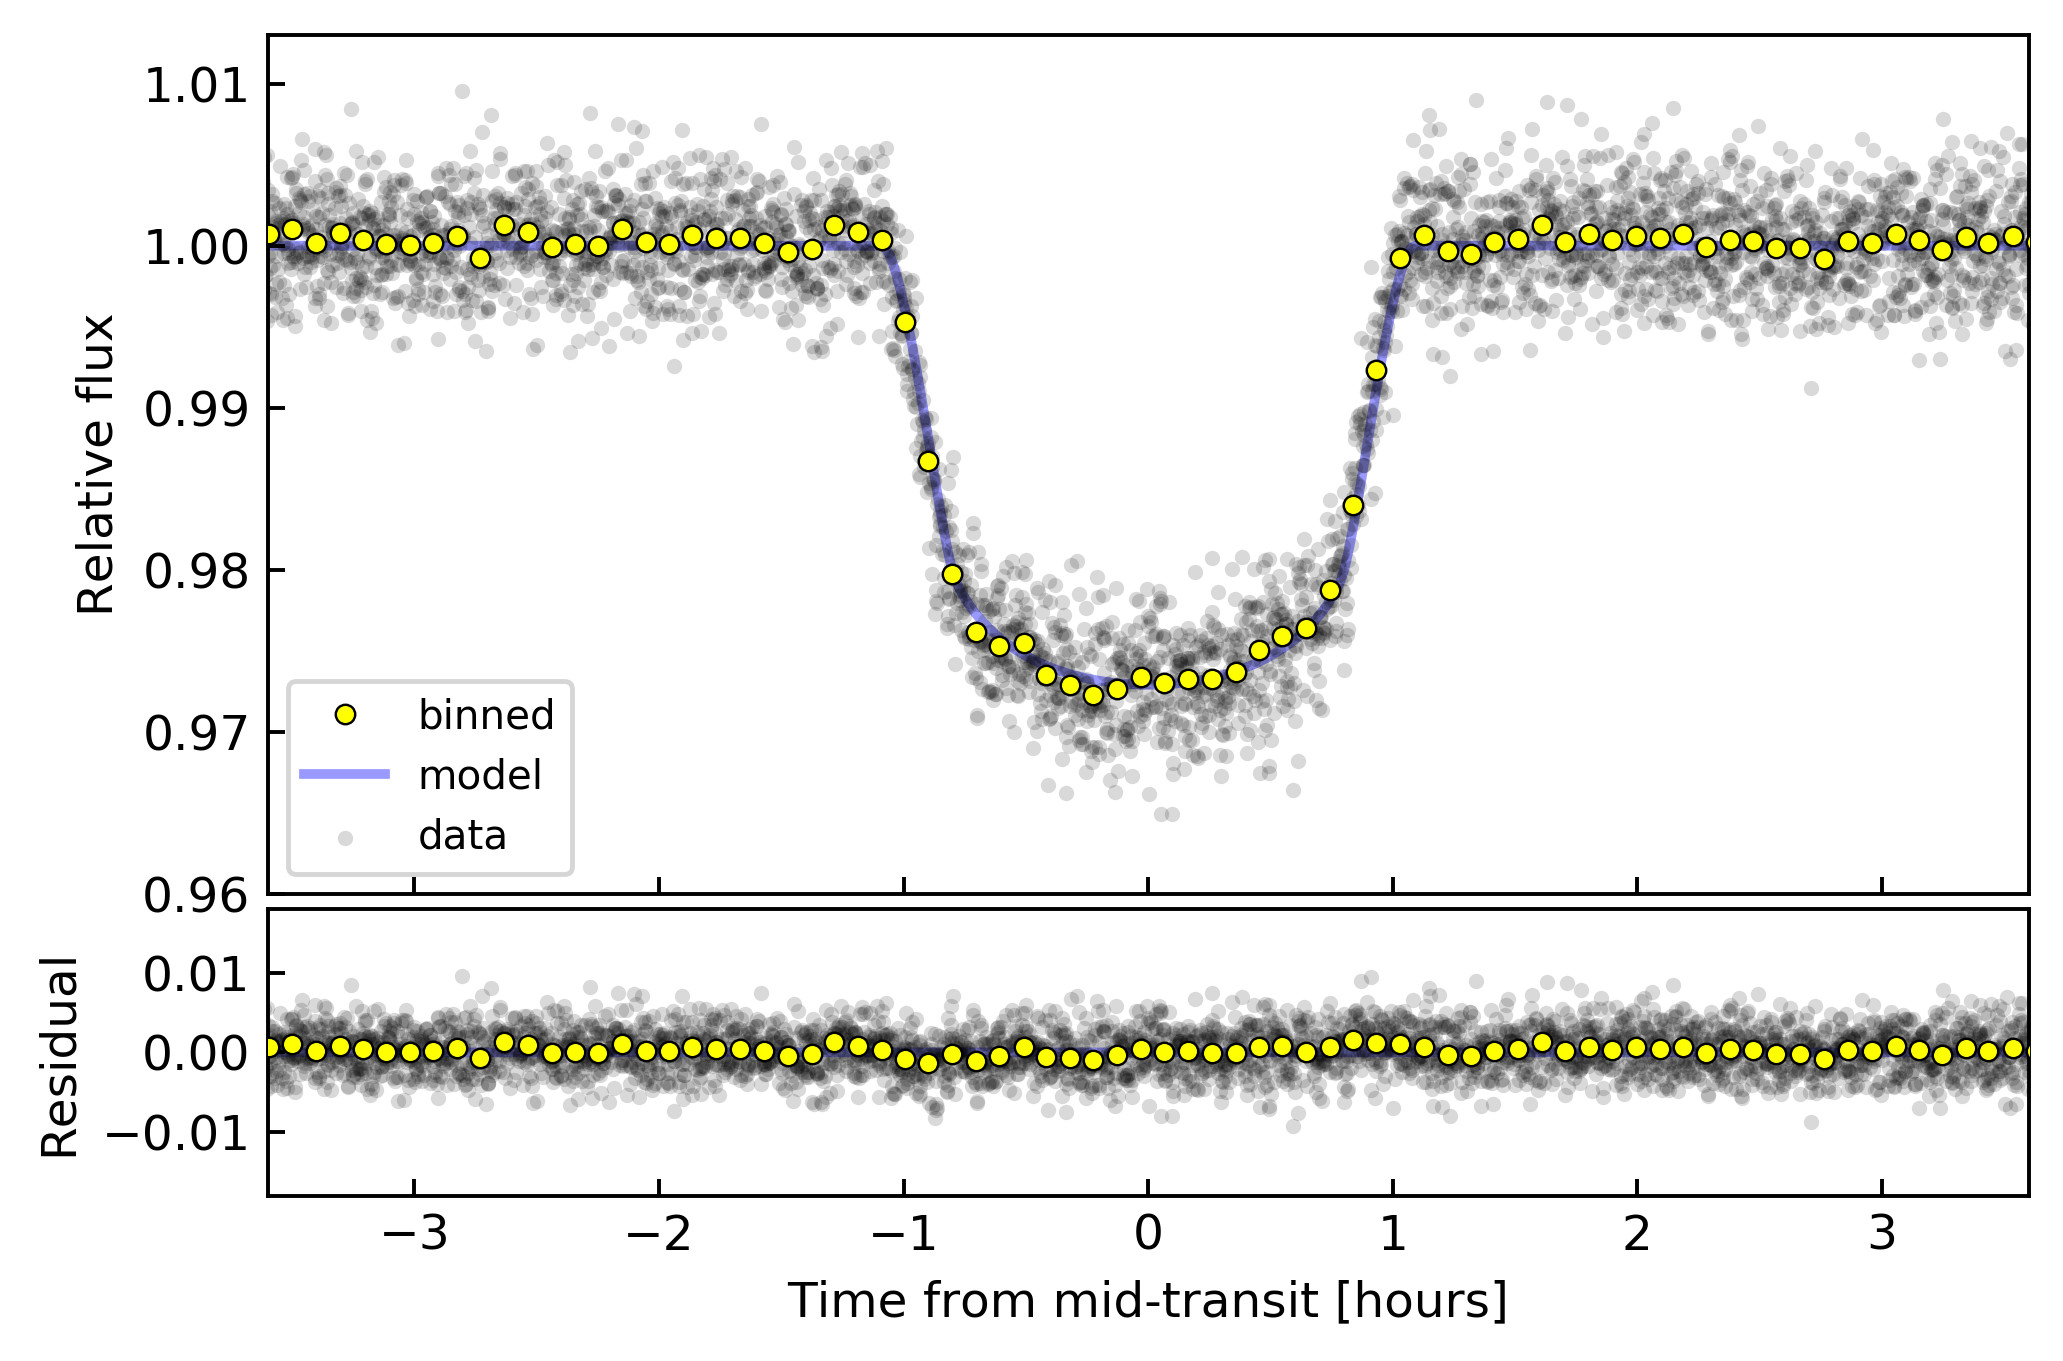
\includegraphics[width=0.48\textwidth]{f1.png}
    \end{center}
    \vspace{-0.5cm}
    \caption{
        {\bf TESS transits of WASP-4b.} On the left, black points are
        TESS flux measurements, with a vertical offset applied. Blue
        curves are best-fit models. Rounded midtimes are printed in
        BTJD next to the appropriate transits.  The residuals are
        shown on the right.
        \label{fig:lightcurves}
    }
\end{figure}

\subsection{Observations}
\label{sec:observations}

WASP-4 was observed in TESS camera 2 from August 23, 2018 to September
20, during the spacecraft's second sector of science operations.  The
star is designated by the TESS Input Catalog as TIC 402026209
\citep{stassun_TIC_2018}.

The TESS spacecraft recorded images of WASP-4 in an $11\times11$ pixel
array every 2 minutes.   After being downlinked through the Deep Space
Network, the data were processed through the Science Processing
Operations Center (SPOC) pipeline at NASA
Ames~\citep{jenkins_tess_2016}.  One important step in this processing
was converting from spacecraft time to barycentric time.  SPOC then
reports timestamps in ``BTJD'', where ${\rm BTJD} = {\rm BJD} -
2457000$, BJD is the barycentric julian date, and all times are in the
TDB reference (see \citealt{urban_explanatory_2012} for explanations
of time systems).  The lightcurves were then vetted and released by
the MIT TESS Science Office to the Mikulski Archive for Space
Telescopes~\citep{ricker_tess_alerts_2018}.

We begin our analysis with the Presearch Data Conditioning (PDC) light
curves from MAST.  The steps used to find an optimal aperture (for
WASP-4, a $3\times 3$ pixel array) and the PDC-MAP algorithm are
described by \citet{smith_kepler_apertures_2017} and
\citet{smith_kepler_PDC_2017} respectively.

We then processed the lightcurve as follows.  First, we removed all
points with non-zero quality flags.  This removes data contaminated by
coarse spacecraft pointing, cosmic rays, and other annoyances
\citep{tess_data_product_description_2018}.  We then filtered out
known bad observing windows.  The data closest to spacecraft perigee
typically show ramp-like systematics, so we clipped out the first and
last hour of both orbits.  Next, we focused on the momentum dumps. As
described in the data release
notes\footnote{\url{archive.stsci.edu/hlsps/tess-data-alerts/hlsp_tess-data-alerts_tess_phot_s01_tess_v1_release-notes.pdf}},
during the first two TESS sectors, every 2.5~days the spacecraft's
reaction wheels were reset to maintain pointing stability.  These
events were assigned quality flags corresponding to ``Reaction Wheel
Desaturation Event'' and ``Manual Exclude''.  For WASP-4, these flags
were simultaneously set for 54 distinct cadences, and there were 10
momentum dumps, averaging about 10 minutes of flagged data per dump.
Simply out of caution, we clipped out an additional 10 minutes before
and after every momentum dump.  Before applying any filters, we had
19737 data points. After applying all the filters, we were left with
18165 measurements, or 92\% of the original data.

After ``cleaning'' the data, we normalized the flux measurements by
dividing out the median flux.  We then converted the timestamps from
BTJD to BJD by adding the appropriate 2457000 day offset
\citep{tess_data_product_description_2018}.  Many of these and
subsequent processing steps were performed using
\texttt{astrobase}~\citep{bhatti_astrobase_2018} We opted not to
``flatten'' the lightcurves at this stage, as is often done with {\it
e.g.}, a spline or gaussian process regression.  Such procedures are
asymmetric about the transit minimum and can skew the transit time
measurement without being captured by the measurement uncertainties.



\subsection{Measuring the transit times}
\label{sec:measurement}

\begin{figure}[t]
    \begin{center}
        \leavevmode
        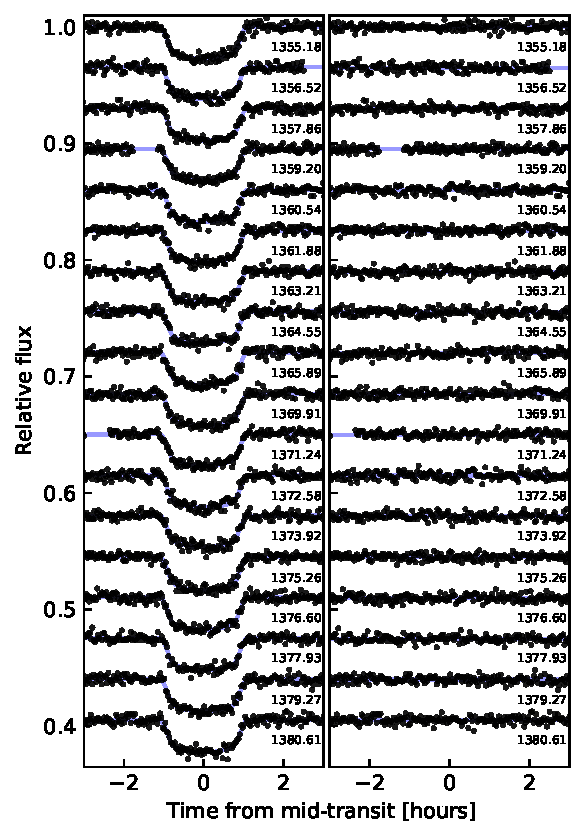
\includegraphics[width=0.48\textwidth]{f2.pdf}
    \end{center}
    \vspace{-0.5cm}
    \caption{
      %TODO: final number
        {\bf TESS saw WASP-4b transit earlier than expected.}
        Points are differences between observed transit times and the
        constant-period ephemeris we fit to literature times.  Black
        points are the more precise half of literature times; gray
        points are the less precise half.  Blue curves represent the
        $\pm 1\sigma$ credible interval around the constant-period
        ephemeris.  The binned TESS observation (red point) arrived
        $77.8 \pm 10.8\ {\rm seconds}$ before it was expected.
        \label{fig:arrived_early}
    }
\end{figure}

Using the cleaned PDC lightcurve, we ran Box Least Squares (BLS) to
estimate the transit epoch, period, and duration
\citep{kovacs_box-fitting_2002}.  Using these parameters, we isolated
each transit to within $\pm$10 transit durations of its midtime.  In
each transit window, we then simultaneously fit for a model transit,
plus a local linear trend.  Our transit model uses the analytic
formulae calculated by \citet{mandel_analytic_2002} and implemented by
\citet{kreidberg_batman_2015}.

We allowed four free parameters per transit: the time of mid-transit
$t_{\rm tra}$, the planet-to-star radius ratio $R_{\rm p}/R_\star$,
and the slope and intercept of the line.
% Our priors were wide uniform distributions centered on the BLS
% estimates for $t_{\rm tra}$ and $R_{\rm p}/R_\star$, and on a slope
% of zero and an intercept of unity for the line.
We fixed the remaining transit parameters as follows.  We set the
eccentricity to zero, and the longitude of periastron to $\pi/2$.  We
assumed a quadratic limb-darkening law, with coefficients interpolated
from the \citet{claret_limb_2017} tables.  For the period,
$a/R_\star$, and inclination, we adopted the values
from~\citet{petrucci_no_2013}.  These are in reasonable agreement with
the parameters reported by \citet{gillon_improved_2009},
\citet{southworth_high-precision_2009}, and
\citet{huitson_gemini_2017}.

Having defined the free and fixed parameters, we calculated an initial
guess for the free parameters by maximizing the likelihood.  We then
sampled over the posterior using the algorithm proposed by
\citet{goodman_ensemble_2010} and implemented by
\citet{foreman-mackey_emcee_2013}.
% During this process, we used the \texttt{corner} software to check
% that our posteriors were being well-sampled~\citep{corner_2016}.
After completing an initial fit, we set the photometric error bars to
be equal to the standard deviation of the in-transit points of the
residual lightcurve.  We then reperformed the fitting procedure, using
the empirically determined photometric errors.

% TODO: final numbers
To verify that the measured uncertainties are plausible, we computed
the reduced $\chi^2$ for a linear ephemeris fit to the measured TESS
transit times.  We found that $\chi^2 = 8.4$, with 16 degrees of
freedom.  Visually inspecting residuals showed that the error variance
had been overestimated, so we multiplied the measured TESS errors by a
factor $f=0.73$, forcing a reduced $\chi^2$ of unity.  This lowered
the mean midtime uncertainty for each transit from 30 to 22 seconds.

Figure~\ref{fig:lightcurves} shows the light curves, best-fit models,
and residuals.  Table~1 reports the mid-transit times and their
uncertainties.  Taking the mean and standard deviation of the measured
planet to star radius ratio, we find $R_{\rm
p}/R_\star=0.1538\pm0.0013$, in agreement with previous determinations
\citep{wilson_wasp-4b_2008,gillon_improved_2009,winn_transit_2009,southworth_high-precision_2009}.
Binning the residuals to 1-hour windows and taking the median absolute
deviation, the lightcurves have a MAD of $594\,{\rm ppm}\,{\rm
hr}^{1/2}$.  The predicted\footnote{\url{github.com/lgbouma/tnm}}
photon-counting noise is $410\,{\rm ppm}\,{\rm hr}^{1/2}$.  At
$T\approx11.8$, with a 9-pixel aperture read noise is expected to
contribute an additional $202\,{\rm ppm}\,{\rm hr}^{1/2}$ in
quadrature.  The predicted zodiacal background contribution is
$673\,{\rm ppm}\,{\rm hr}^{1/2}$, based on the
\citet{winn_photonflux_2013} model, which \citet{Sullivan_2015} used
in planet detection simulations.  This zodiacal noise prediction seems
to have been an overestimate, given the observed MAD of WASP-4.  A
more detailed assessment of TESS's photometric performance is beyond
the scope of this work.


\subsection{Star and planet parameters}
\label{sec:system_parameters}

\begin{deluxetable}{lccc}
\tabletypesize{\scriptsize}
\tablecaption{Selected system parameters of WASP-4b\label{tbl:params}}
\tablenum{2}

\tablehead{
\colhead{Parameter} & \colhead{Value} & \colhead{Error} & \colhead{Comment}
}

\startdata
{\it Transit/RV parameters:} & & & \\
  $R_{\rm p}/R_\star$                        & $0.1538$               & $\pm 0.0013$                & A \\
  $i$~[deg]                                  & $88.52$                & $+0.39$, $-0.26$            & B \\
  $a/R_\star$                                & $5.463$                & $+0.025$, $-0.020$          & B \\
  $K$~[m~s$^{-1}$]                           & $241.1$                & $+2.8$, $-3.1$              & C \\
{\it Stellar parameters:} & & & \\
  $T_{\rm eff}$~[K]                          & $5400$                 & $\pm 90$                    & D \\
  $\log g_\star$~[cgs]                       & $4.47$                 & $\pm 0.11$                  & D \\
  $[{\rm Fe/H}]$                             & $-0.07$                & $\pm 0.19$                  & D \\
  $F_{\rm bol}$~[erg~cm$^{-2}$~s$^{-1}$]     & $2.802\times10^{-10}$  & $\pm 0.076\times10^{-10}$   & E \\
  $\pi$~[mas]                                & $3.7145$               & $0.0517$                    & G \\
  $R_\star$~[R$_{\odot}$]                    & $0.893$                & $\pm 0.034$                 & F \\
  $\rho_\star$~[g~cm$^{-3}$]                 & $1.722$                & $+0.024$, $-0.019$          & A \\
  $M_\star$~[M$_{\odot}$]                    & $0.870$                & $+0.085$, $-0.077$          & F \\
  $T$ magnitude                              & $11.778$               & $\pm 0.018$                 & H \\
{\it Planetary parameters:} & & & \\
  $a$~[AU]                                   & $0.0227$               & $\pm 0.0007$                & F \\
  $M_p$~[M$_{\rm Jup}$]                      & $1.192$                & $+0.091$, $-0.086$          & F \\
  $R_p$~[R$_{\rm Jup}$]                      & $1.337$                & $\pm 0.048$                 & F \\
\enddata

\tablecomments{
  (A) From TESS lightcurves (\S~\ref{sec:measurement}).
  (B) \citet{hoyer_tramos_2013}.
  (C) \citet{triaud_spin-orbit_2010}.
  (D) From HARPS spectra \citep{doyle_accurate_2013}.
  (E) \citet{stassun_accurate_2017}.
  (F) From functions of stellar, transit or RV parameters as discussed in text.
  (G) {\it Gaia} DR2.
  (H) \citet{stassun_TIC_2018}.
}

\end{deluxetable}

\citet{doyle_accurate_2013} found accurate spectroscopic parameters
for WASP-4 using high S/N HARPS spectra.  Using their (T$_{\rm eff}$,
$\log g$, $[{\rm Fe/H}]$) and the available {\it Gaia} parallaxes, we
compute the remaining system parameters empirically.

We compute the bolometric flux using broadband magnitudes from
available all-sky catalogs, as follows: $G$ from {\it Gaia\/} DR2,
$B_T V_T$ from {\it Tycho-2}, $BVgri$ from {\it APASS}, $JHK_S$ from {\it
2MASS}, and the {\it WISE}~1--4 passbands, thus spanning the
wavelength range 0.4--22~$\mu$m.  Combining the implied angular radius
with the {\it Gaia} DR2 parallax, and adjusting for the parallax
offset \citep{stassun_evidence_2018}, we obtain the stellar radius.
For the stellar mass, we started with the $a/R_\star$ value found by
\citet{hoyer_tramos_2013} from 26 ground-based transits.  The implied
semi-major axis and stellar density follow \citep{seager_unique_2003}.
Combining the density and radius gives the stellar mass.  We get the
planet radius using our measured $R_{\rm p}/R_\star$.  Finally, for
the planet mass we use the observed RV semi-amplitude and inclination
angle from the transit
\citep{triaud_spin-orbit_2010,hoyer_tramos_2013}.

The resulting parameters are in Table~3, and broadly agree with those
of previous authors
\citep{wilson_wasp-4b_2008,gillon_discovery_2009,winn_transit_2009,southworth_homogeneous_2011,petrucci_no_2013}.
We use them for the remaining analysis.  Comparing the empirical
result to the Yonsei-Yale evolutionary track predicted by the
spectroscopic parameters, we see that WASP-4  has an age $\approx
7\,{\rm Gyr}$, and is securely in the main-sequence stage of
evolution.

\section{Timing analysis}
\label{sec:timing}

\subsection{Previous timing measurements}
\label{subsec:times}

\begin{figure*}[t]
    \begin{center}
        \leavevmode
        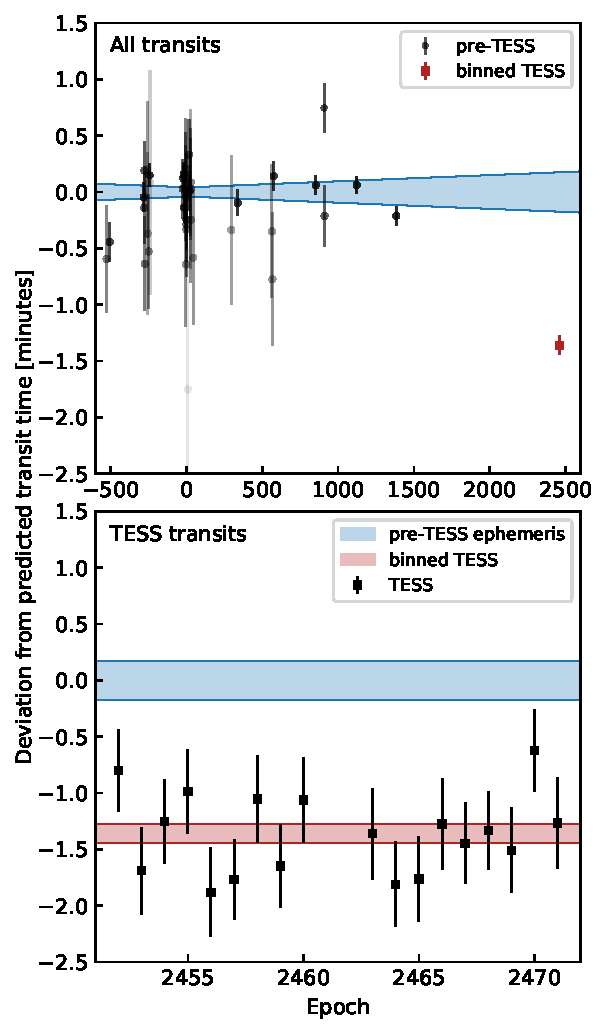
\includegraphics[width=0.9\textwidth]{f3.pdf}
    \end{center}
    \vspace{-0.5cm}
    \caption{
        {\bf Timing residuals and best-fit models for WASP-4b.}
        Points are differences between observed transit times and a
        linear ephemeris fit to all the times.  The constant period
        model is a poor fit to the observed times (gray line).  Black
        points are the more precise half of measured times; gray
        points are the less precise half.  The blue curve is the
        best-fit model with a constant period derivative.  The orange
        curve is the best-fit model assuming apsidal precession causes
        the observed timing deviations. The binned TESS point (star)
        is for display purposes only.
        \label{fig:times}
    }
\end{figure*}

Table~1 shows the transit times used in our analysis.  We included
data from peer-reviewed literature for which the analysis was based on
observations of a single, complete transit, and for which the midpoint
was fit as a free parameter. We also required that the time system be
clearly documented.  The occultation times are in Table~3.  Since
there are fewer available, we included all the occultation
measurements we could find. The tabulated values have been corrected
for the light-travel time across the diameter of the orbit by
subtracting $2a/c = 22.8$ seconds from the observed time.

We used the homogeneous \citet{hoyer_tramos_2013} timing study as our
starting point.  Though their latest two epochs fell slightly below
the prediction of a linear ephemeris (Panel C of their Figure~6), they
did not find a need to fit a quadratic function to the O-C values.  We
verified that all times were on the BJD$_{\rm TDB}$ time standard
using the \citet{eastman_achieving_2010} calculator.  We set the
zero-point epoch to be as close as possible to the average of the
midtimes, weighted as the inverse midtime variance. This minimizes the
covariance between the transit epoch and the period
\citep{gibson_gemini_2013}.

Important contributions to the timing dataset are as follows.  Our
earliest epoch is from EulerCam on the 1.2-m Euler telescope
\citep{wilson_wasp-4b_2008}.  The second epoch comes from $z$-band
photometry acquired by \citet{gillon_improved_2009} at the VLT 8.2-m
with FORS2.  Subsequent transits came from
\citet{winn_transit_2009}\footnote{\citet{winn_transit_2009} recorded
the GPS clock time in UT reference. They then converted this to BJD in
the TDB reference for their reported midtimes.},
\citet{dragomir_terms_2011}, \citet{sanchis-ojeda_starspots_2011},
\citet{nikolov_wasp-4b_2012}, \citet{hoyer_tramos_2013}, and
\citet{ranjan_atmospheric_2014}.  Finally, \citet{huitson_gemini_2017}
acquired optical transmission spectra with the 8.1-m Gemini South
telescope over 2011 to 2014, one transit per season.  The per-point
standard deviation of their lightcurves is a few hundred parts per
million, within a factor of 3 from the photon noise limit.  The
uncertainties on their reported transit times~--~on average
5.6~seconds~--~ are small, but possible given the quality of their
data~\citep{carter_analytic_2008}.

%%%%%%%%%%%%%%%%%%%%%%%%%%%%%%%%%%%%%%%%%%
%\citet{winn_transit_2009} measured two transits with the Baade 6.5-m
%at Las Campanas\footnote{\citet{winn_transit_2009} recorded the GPS
%clock time in UT reference. They then converted this to BJD in the
%TDB reference for their reported midtimes.}, and reported transit
%midtimes precise to 6~seconds.  \citet{dragomir_terms_2011} updated
%the ephemeris using two transits measured with the CTIO 0.9-m and
%1.0-m.  \citet{sanchis-ojeda_starspots_2011} reported four more
%transits from the Baade telescope at Las Campanas\footnote{
%\citet{sanchis-ojeda_starspots_2011} also used starspot occultations
%to show that the star's rotation axis is nearly aligned with the
%planet's orbital axis, in agreement with the Rossiter-McLaughlin
%measurement by \citet{triaud_spin-orbit_2010}.}.
%\citet{nikolov_wasp-4b_2012} observed 3 transits, in 4 independent
%photometry bands (Sloan {\it g'}, {\it r'}, {\it i'}, {\it z'}) with
%the MPG/EOS-2.2~m at La Silla.  \citet{hoyer_tramos_2013} reported
%nine transit observations taken with the the Y4KCAM on the SMARTS 1-m
%telescope, and another three with the SOI on the SOAR 4.2-m
%telescope.  \citet{hoyer_tramos_2013} also homogeneously redetermined
%the transit times from all previous studies.  After the study by
%\citet{hoyer_tramos_2013}, \citet{ranjan_atmospheric_2014} acquired
%near-IR spectra of WASP-4b using HST's WFC3 in both transit and
%secondary eclipse.  We adopt only their transit time, since the epoch
%of occultation was not fit as a free parameter.'

% There have been other studies of WASP-4b for which the transit
% timing data are either hetereogenous, not available, or not useable.
% We omitted the timing measurements from
% \citet{southworth_high-precision_2009}, since there were technical
% problems with the computer clock at the time of
% observation~\citep{nikolov_wasp-4b_2012}.  The timing study
% by~\citet{petrucci_no_2013} ruled out transit timing variations
% larger than 54~seconds over the previous 5 years, but did not report
% transit times.  \citet{baluev_benchmarking_2015} collected transit
% times for many hot Jupiters, including WASP-4b, and included times
% from the Exoplanet Transit Database
% (ETD)\footnote{\url{http://var2.astro.cz/ETD/}}
% \citep{poddany_ETD_2010}.  Since the ETD data come from
% heterogeneous sources, their timestamps are less clearly documented,
% and the times are thus more prone to systematic errors, we omit them
% from consideration.  %We consider the effects of including ETD data
% in %Appendix~\ref{sec:verify_archival_times}.
% \citet{may_mopss_2018} obtained optical spectra using IMCAS on
% Magellan, and found a flat transmission spectrum, in agreement with
% the results reported by \citet{huitson_gemini_2017}.  They did not
% report transit times.
%%%%%%%%%%%%%%%%%%%%%%%%%%%%%%%%%%%%%%%%%%

There are fewer available occultation times.
\citet{beerer_secondary_2011} observed two occultations of WASP-4b
using warm Spitzer in the 3.6\,$\mu$m and 4.5\,$\mu$m bands.
\citet{caceres_ground-based_2011} detected an occultation from the
ground in the ${\rm K}_{\rm s}$ band, and gave a time in HJD, without
specifying the time standard.  We correspondingly added $69.184$
seconds of uncertainty to their reported errors, in quadrature.
%Finally, as previously mentioned, \citet{ranjan_atmospheric_2014}
%acquired occultation data with HST but kept the epoch as a fixed
%parameter.
\citet{zhou_secondary_2015} acquired occultation data from the
Anglo-Australian Telescope, focusing on the eclipse depth, but also
fitting for $e\cos\omega$.  We converted their $e\cos\omega$ result
into a midtime, using their ephemeris and the standard formula
\citep[{\it e.g.},][]{winn_exoplanet_2010}
\begin{equation}
  t_{\rm occ}(E) =
  t_0 +  P E  +
  \frac{P}{2} \left( 1 + \frac{4}{\pi} e\cos\omega \right).
  \label{eq:occultation_time}
\end{equation}
This gives us a total of 4 occultations.  Although the occultation
times are uncertain compared to the transits, they nonetheless help in
modeling the timing variations.

\subsection{Analysis}

After collecting the literature times and measuring the TESS times, we
compared the observed time to the prediction based solely on the
literature times. The result is shown in
Figure~\ref{fig:arrived_early}. The TESS observations 
arrived early.  One immediate concern was systematic errors in either
the archival or the TESS timestamps. The tests we used to mitigate the
latter possibility are described in Appendix~\ref{sec:verify_tess}.

Assuming that the observed timing variation is astrophysical, we
proceeded by exploring three models for the timing data, identical to
the study by~\citet{patra_2017}.  

The first model assumes a constant orbital period on a circular orbit:
\begin{align}
  t_{\rm tra}(E) &= t_0 + PE,\\
  t_{\rm occ}(E) &= t_0 + \frac{P}{2} + PE,
\end{align}
for $E$ the epoch number.
The two free parameters are the reference epoch $t_0$ and the period $P$.

The second model assumes a constant period derivative, and a circular
orbit:
\begin{align}
  t_{\rm tra}(E) &=
    t_0 + PE +
    \frac{1}{2} \frac{{\rm d}P}{{\rm d}E} E^2, \\
  t_{\rm occ}(E) &=
    t_0 + \frac{P}{2} + PE +
    \frac{1}{2} \frac{{\rm d}P}{{\rm d}E} E^2.
\end{align}
The three free parameters are the epoch, period at the reference epoch,
and period derivative, ${\rm d}P/{\rm d}t = (1/P) {\rm d}P/{\rm d}E$. 

The third model assumes the planet has a slightly eccentric orbit, and
that the line of apsides is rotating:
\begin{align}
  t_{\rm tra}(E) &= 
		t_0 + P_{\rm s}E
    - \frac{e P_{\rm a}}{\pi} \cos\omega,\\
  t_{\rm occ}(E) &= 
    t_0 + \frac{P_{\rm a}}{2} + P_{\rm s}E
    + \frac{e P_{\rm a}}{\pi} \cos\omega,
\end{align}
for $P_{\rm s}$ the sidereal period, $e$ the eccentricity, $P_{\rm a}$
the anomalistic period, and $\omega$ the argument of pericenter.
Following~\citet{gimenez_revision_1995} and~\citet{patra_2017}, in
this model the angular velocity of the line of apsides ${\rm
d}\omega/{\rm d}E$ is constant,
\begin{equation}
  \omega(E) = \omega_0 + \frac{{\rm d}\omega}{{\rm d}E} E,
\end{equation}
and the sidereal and anomalistic periods are related by
\begin{equation}
  P_{\rm s} = P_{\rm a} \left(
    1 - \frac{1}{2\pi}\frac{{\rm d}\omega}{{\rm d}E}
    \right).
\end{equation}
The five free parameters are the epoch, sidereal period, eccentricity,
argument of pericenter at the reference epoch, and angular velocity of
line of apsides:
$(t_0, P_{\rm s}, e, \omega_0, {\rm d}\omega/{\rm d}E)$.

%%%%%%%%%%%%%%%%%%%%%%%%%%%%%%%%%%%%%%%%%%
% Assuming the error bars on the transit midtimes are gaussian and
% independent, we then proceed by fitting each model to the timing data.
% For the linear model, we took uniform priors over small windows around
% the expected parameters.  For the quadratic model we did the same, and
% took the quadratic term to have a uniform prior corresponding to
% $
%   Q_\star' \sim \mathcal{U}[10^3, 10^9],
% $
% for $Q_\star'$ the modified quality factor defined in
% \S~\ref{sec:implications}.  For the precession model, we took the same
% priors in epoch and sidereal period, and drew the remaining parameters
% from wide uniform distributions.
%%%%%%%%%%%%%%%%%%%%%%%%%%%%%%%%%%%%%%%%%%

%TODO: final numbers
Figure~\ref{fig:times} shows the residuals with respect to the linear
model.  The best linear fit has $\chi^2 = 149$ and 58 degrees of
freedom.  The best quadratic fit has $\chi^2 = 48.0$ and 57
degrees of freedom, compared to $\chi^2 = 51.0$
and 55 degrees of freedom for the best-fit precession model.

%TODO: final numbers
The difference in $\chi^2$ between the linear and quadratic fit
corresponds to $p \approx 10^{-23}$.  Clearly, it is more likely that
some systematic error could be affecting one of the most important
sets of times: either the earliest times, the Huitson et al.\ Gemini
times (epoch numbers 44, 322, 591, and 851), or the TESS times.  We
have taken every precaution against systematic offsets in the TESS
dataset (Appendix~\ref{sec:verify_tess}). Huitson et al.\ stand by
their reported times (J.-M. D\'esert, priv.\
comm.)\footnote{\citealt{huitson_gemini_2017} corrected the times to
be at mid-exposure. They also analyzed other hot Jupiters, which all
showed mid-transit times as expected from a constant ephemeris.}.
Since the linear model provides a poor fit to the data, we discard it
from further consideration.

%TODO: final numbers
The quadratic model fits better than the precession model.  It is
favored by $\Delta \chi^2 = 3.0$, and has two fewer free parameters.
Another useful heuristic for model comparison is the Bayesian
Information Criterion (BIC),
\begin{equation}
  {\rm BIC} = \chi^2 + k\log n,
\end{equation}
for $k$ the number of free parameters, and $n$ the number of data
points. For us, $n=60$.  The difference in the BIC for the precession
and decay models is $\Delta {\rm BIC} = {\rm BIC}_{\rm prec} - {\rm
BIC}_{\rm quad} = 11$, corrsonding to a Bayes factor of $\approx
4\times10^{4}$.  The Akaike Information Criterion
similarly favors the orbital decay model, by $\Delta {\rm AIC} = 7$.
This is strong evidence that the quadratic model describes the
data better than the precession model \citep{kass_bayes_1995}.

%TODO: final numbers
If we assume the orbital decay model, we find a period derivative 
\begin{equation}
\dot{P}
  = - (3.82 \pm 0.38)\times 10^{-10}
  = - (12.1) \pm 0.12\,{\rm ms}\,{\rm yr}^{-1}.
  \label{eq:dP_dt_obs}
\end{equation}
For comparison, the period derivative seen by
\citet{maciejewski_departure_2016} and \citet{patra_2017} in WASP-12b
is $\dot{P} = -29 \pm 3\,{\rm ms}\,{\rm yr}^{-1}$.  If both planets
are decaying, WASP-4b would be inspiraling at about half the rate as
WASP-12b.

%TODO: final numbers
If we instead assume the precession model, the best-fit eccentricity
is
\begin{equation}
  e = (1.63^{+ 1.48}_{- 0.65})\times10^{-3}
\end{equation}
The longitude of periapse correspondingly advances by $\dot{\omega}
= 14.8^{+5.4}_{-3.8}\ {\rm degrees}\,{\rm yr}^{-1}$, and the
precession period would be $24^{+8}_{-6}$ years.

The median parameters and their standard deviations are reported for
the three models in Table~4.  In short, a linear ephemeris does not
describe the observed times.  Both orbital decay and precession can
fit the data, but the precession model is statistically disfavored.


\section{Implications}
\label{sec:implications}

\begin{figure}[t!]
  \begin{center}
    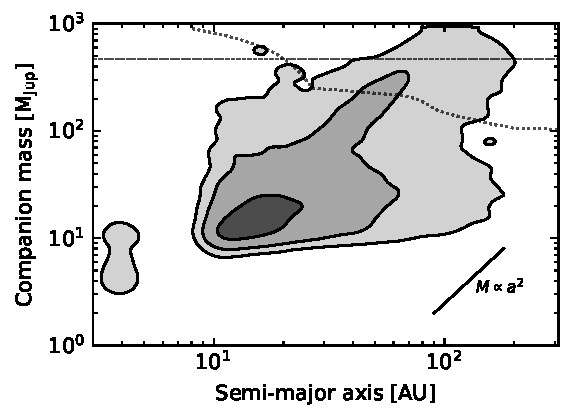
\includegraphics[width=0.425\textwidth]{f4.pdf}
  \end{center}
  \vspace{-0.5cm}
  \caption{
    {\bf WASP-4b has a short eccentricity damping time and medium
    decay time compared to other hot Jupiters.  It seems to orbit a
    main sequence host.
    }
    {\bf \it Top:}
    Transiting giant planets from \citet{bonomo_gaps_2017}, who
    measured the eccentricities using radial velocities.  Solid
    squares (including WASP-18b) have significant eccentricity
    detections.  The axes are chosen so that constant eccentricity
    damping timescales (Equation~\ref{eq:de_dt}) are lines.  The
    contours shown assume $Q_{\rm p}' = 10^5$.
    {\bf \it Middle:} 
    Axes are chosen so to that constant orbital decay timescales
    (Equation~\ref{eq:da_dt}) are lines.  The contours shown assume
    $Q_\star' = 10^7$.
    {\bf \it Bottom:}
    HR diagram highlighting WASP-12b, which shows timing variations
    similar to WASP-4b.  We also show hot Jupiters for which we
    detect no timing variation (see \S~\ref{sec:hj_verification}).
    \label{fig:context}
  }
\end{figure}

 
\subsection{Orbital decay}

The middle panel of Figure~\ref{fig:context} shows the expected
orbital decay time of WASP-4b compared to other transiting giant
planets.  Though roughly 20 hot Jupiters might be expected to decay
faster, some orbit stars with minimal convective zones ({\it e.g.},
WASP-18), and most are not as well-observed as WASP-4.

For the sake of argument, let us assume that the timing variation is
caused entirely by orbital decay.  If the period continues to decrease
at a fixed rate, it will reach zero after
\begin{equation}
  \frac{P}{ \dot{P} } = 9.6 \, {\rm Myr}.
\end{equation}
For comparison, the ``survival time'' found by \citet{patra_2017} for
WASP-12b was 3.2\,Myr.

Let us assume further that the ``constant phase lag'' model for tidal
interaction in a binary applies \citep{zahn_tidal_1977}.  The fluid
response is parametrized by a modified\footnote{For stars, $k_\star
\sim \mathcal{O}(10^{-2})$, so it is important to explicitly
distinguish $Q_\star'$ from $Q_\star$ \citep[{\it
e.g.},][]{schwarzschild_structure_1958}.} quality factor, $Q_\star' =
3 Q_\star / (2k_\star)$.  Here $k_\star$ is the stellar Love number,
which is smaller when the star's density distribution is more
centrally concentrated. $Q_\star$ is the ratio of the energy stored in
the equilibrium deformation of the star, divided by the energy lost to
heat per tidal period \citep[{\it e.g.},][]{goldreich_q_1966}.  A
larger $Q_\star$ implies less efficient dissipiation.  Though the
fluid mechanics responsible for the dissipation should depend on the
amplitude and frequency of the tidal perturbation
\citep[][Section~3.3]{ogilvie_tidal_2014}, we will treat $Q_\star'$ as
a constant.  This should not be taken literally; $Q_\star'$ may in
fact change sharply with varying tidal frequency
\citep{penev_empirical_2018}.

If the planet's spin and orbit are synchronized, the star is slowly
rotating, and the eccentricity is small, then the semi-major axis and
eccentricity evolve as \citep[Appendix B of][]{metzger_optical_2012}
\begin{align}
  \frac{1}{\tau_{\rm e}} &=
  \frac{|\dot{e}|}{e} =
    \frac{63 \pi } {2 Q_{\rm p}' }
    \left( \frac{R_{\rm p}}{a} \right)^5
    \left( \frac{M_\star}{M_{\rm p}} \right)
    \left( \frac{1}{P} \right)
  \label{eq:de_dt}
  \\
  \frac{1}{\tau_{\rm a}} &=
  \frac{|\dot{a}|}{a} =
    \frac{9 \pi } {Q_\star' }
    \left( \frac{R_\star}{a} \right)^5
    \left( \frac{M_{\rm p}}{M_\star} \right)
    \left( \frac{1}{P} \right).
  \label{eq:da_dt}
\end{align}
The orbital period evolves as
\begin{equation}
\label{eq:dP_dt}
  \dot{P} = -\frac{27\pi}{2 Q_\star'}
            \left(\frac{M_{\rm p}}{M_\star}\right)
            \left(\frac{R_\star}{a}\right)^5.
\end{equation}
Using the observed value of $\dot{P}$, the current modified quality
factor of WASP-4 would be
\begin{equation}
	Q_\star' \approx 3.3\times10^4. 
\end{equation}
This is rather small.  Jupiter has $Q_{\rm Jup}' \approx 1.4 \times
10^5$, based on the orbits of the Galilean moons
\citep{lainey_strong_2009}.  For stars, studies of the binary
eccentricity distribution have yielded $Q_\star' \approx 10^5 - 10^7$
\citep[{\it e.g.},][]{meibom_robust_2005,belczynski_compact_2008,
geller_direct_2013,milliman_wiyn_2014}.  However the dissipation rates
may differ in hot Jupiter systems, since the tidal forcing frequencies
and amplitudes are different.  Observationally-driven studies of hot
Jupiter systems have found $Q_\star' \approx 10^5 - 10^8$, often using
different models
\citep{jackson_observational_2009,hansen_calibration_2010,penev_constraining_2012,penev_empirical_2018,cameron_hierarchical_2018}.
For instance, motivated by the rapid rotation of some hot Jupiter
hosts \citep{pont_empirical_2009,penev_hats-18b_2016},
\citet{penev_empirical_2018} modeled the evolution of hot Jupiter
systems under the influence of a magnetized wind and a constant
phase-lag tide.  For WASP-4, their method gave $Q_\star' \approx
(1.2^{+1.0}_{-0.5})\times10^7$.  This disagrees strongly with the
value we infer from the apparent period change.

%%%%%%%%%%%%%%%%%%%%%%%%%%%%%%%%%%%%%%%%%%
% In fact, for the observed population of hot Jupiters,
% \citet{penev_constraining_2012} argued that $Q_\star' > 10^7$ would
% be required at some phase of hot Jupiter evolution at the 99\%
% level, or else the observed population would not exist (though
% \citealt{birkby_wts-2_2014} point out more efficient dissipation
% would be allowed if the hot Jupiters arrived later).  Developing a
% generative model for the orbital separation distribution of the hot
% Jupiter population, \citet{cameron_hierarchical_2018} similarly
% found $10^7 \gtrsim Q_\star' \gtrsim 10^8$.

% Using an empirical approach, \citet{penev_empirical_2018} reported a
% $Q_\star'$ measurement for WASP-4.  In earlier work,
% \citet{penev_hats-18b_2016} noted that HATS-18b and WASP-19b orbited
% host stars whose isochronal ages are consistent with the Sun, but
% whose stellar rotation periods are about 10 days
% (\citealt{pont_empirical_2009} pointed out similar evidence for hot
% Jupiter host spin-up).  The expected rotation periods at solar ages
% are 20 to 30 days
% (\citealt{schatzman_theory_1962,skumanich_time_1972}, and
% measurements by \citealt{barnes_rotation_2016} in the 4\,Gyr-old M67
% cluster).  Assuming that the difference between the observed and
% predicted stellar rotation period was due to tides depositing
% angular momentum in the star, \citet{penev_empirical_2018} modeled
% the evolution of hot Jupiter systems under the influence of a
% magnetized wind and a constant phase-lag tide.  They found two-sided
% limits for $Q_\star'$ in 35 of the 188 systems they examined.  In
% these 35 systems, they found that $Q_\star'$ varied from $10^5$ at
% tidal periods of 2 days to $10^7$ at tidal periods of 0.5 days.  For
% WASP-4 specifically, their method gave $Q_\star' \approx
% (1.2^{+1.0}_{-0.5})\times10^7$. This is more than 2 orders of
% magnitude less efficient than the dissipation rate inferred from the
% decaying orbit would imply.
%%%%%%%%%%%%%%%%%%%%%%%%%%%%%%%%%%%%%%%%%%

A theoretically-motivated model for tidal dissipation was proposed by
\citet{essick_orbital_2016}, who considered the nonlinear response of
the star to a coupled network of gravity modes excited at the base of
the convective zone, and braking near the stellar core.  In their
approach, the stellar quality factors in hot Jupiter systems vary from
$Q_\star' \approx 10^5 - 10^6$.  Using their Equation 26, the
prediction for WASP-4 is $Q_\star' = 7\times10^5$.  This is an order
of magnitude larger than implied by the observed period change.

The applicability of the \citet{essick_orbital_2016} model depends on
the evolutionary state of the star.  The bottom panel of
Figure~\ref{fig:context} shows WASP-4 in the context of other giant
planet hosts from the \citet{bonomo_gaps_2017} sample.  On the y-axis
is $G=g-\mu$, for $g$ the apparent Gaia-band magnitude, and $\mu$ the
distance modulus reported by \citet{gaia_collaboration_gaia_2018}.
The x-axis is the effective temperature from \citet{bonomo_gaps_2017},
which for WASP-4 agrees within $1\sigma$ of that from Table~2.
Inspecting the HR diagram, WASP-4 shows litle evidence of being
evolved, in agreement with our analysis from
\S~\ref{sec:system_parameters}.
%%%%%%%%%%%%%%%%%%%%%%%%%%%%%%%%%%%%%%%%%%
% By a similar argument though, WASP-12 would not clearly stand out as a
% candidate subgiant, and \citet{weinberg_tidal_2017} suggest it may in
% fact be a subgiant (though \citealt{bailey_understanding_2019} do not
% find evidence that supports this suggestion).  A more thorough
% isochronal analysis would be of interest, particularly if the transit
% and occultation times continue to vary.  Such an analysis is beyond
% the scope of this study.
%%%%%%%%%%%%%%%%%%%%%%%%%%%%%%%%%%%%%%%%%%

In short, if the observed period change is caused entirely by tidal
decay, it would imply a tidal dissipation efficiency stronger than
most predictions.  It might be possible that we are observing at a
special time, shortly after the planet's inward migration, or when the
planet is near resonance with a stellar oscillation mode
\citep{ogilvie_tidal_2014,essick_orbital_2016}.  Tidal dissipation
rates might also be increased if the star is turning off the main
sequence.  All of these explanations are strained; it is unclear that
tidal decay could explain the observed timing variations without
fine-tuning.


\subsection{Apsidal precession}
\label{sec:apsidal_precession}

Let us instead assume that the timing variation can be explained as
being a portion of an apsidal precession cycle.  The required orbital
eccentricity is then $e\approx 1.6\times10^{-3}$, and one full
precession period would take about 24 years.

\citet{ragozzine_probing_2009} calculated apsidal precession periods
for hot Jupiters ranging between of order 10 and 100 years.  They
highlighted that for many hot Jupiters, including WASP-4b, over 90\%
of the apsidal precession comes from the tidal bulge of the planet.
Precession from general relativity, the planet's rotational bulge, and
the star's rotational and tidal bulges are minor additions.
%\citet{ragozzine_probing_2009} also calcuated that WASP-4b was expected
%to have a relatively short precession period, of 120 years.

\citet{ragozzine_probing_2009} also noted that if the planet has
non-zero eccentricity, a measurement of $\dot{\omega}$ can be used to
measure the planet's Love number, $k_{2,\rm p}$.  From their Equation
14, the implied Love number for WASP-4b is
\begin{equation}
k_{2,{\rm p}} = 1.6^{+2.1}_{-1.2}.
\end{equation}
For comparison, $k_{2,{\rm Jup}} \approx 0.55$
\citep{wahl_tidal_2016,ni_empirical_2018}.  A uniform density sphere
has $k_2 = 1.5$.  The uncertainties on $k_{2,{\rm p}}$ are large
because the eccentricity, reference time, and ${\rm d}\omega/{\rm d}E$
are correlated, and the measured occultation times only barely
constrain them (Figure~\ref{fig:future}).

\subsubsection{Observations of small eccentricities in hot
Jupiter systems}

Could the eccentricity truly be non-zero?  For WASP-4b, the
eccentricity damping timescale (Equation~\ref{eq:de_dt}) is $\tau_e =
0.29 (Q_{\rm p}'/10^5) \, {\rm Myr}$.  The system is well over
$1\,{\rm Gyr}$ \citep{winn_transit_2009} old, so any initial
eccentricity should have been erased.

The top panel of Figure~\ref{fig:context} compares the expected
eccentricity damping time of WASP-4b with other transiting giant
planets.  WASP-4b has one of the shortest known eccentricity damping
times.  The hot Jupiter with the nearest $\tau_e$ and a significant
measured eccentricity is WASP-18b, with $e = 0.0076 \pm 0.0010$
\citep{triaud_spin-orbit_2010,bonomo_gaps_2017}.  This is the smallest
significant eccentricity measured by the RV method, with the
next-smallest cases being HAT-P-20b ($e =
0.01580^{+0.0023}_{-0.0018}$), and WASP-38b ($e =
0.02780^{+0.003}_{-0.0028}$).
% For the 231 planets studied by \citet{bonomo_gaps_2017}, 2 (13) had
% $2\sigma$ upper limits of $e < 0.01$ ($e<0.02$).  For WASP-4b, the
% strongest $2\sigma$ upper-limit on its eccentricity from RVs is
% $e<0.011$ \citep{husnoo_observational_2012,bonomo_gaps_2017}.  

Occultation timing can provide stronger eccentricity limits than RV
measurements, but they often come with caveats.  For WASP-4b, the
strongest limit on its eccentricity comes from
\citet{beerer_secondary_2011}, who observed occultations and derived a
$2\sigma$ upper limit on $| e\cos\omega | $ of 0.0024.
% \citet{caceres_ground-based_2011} report $e\cos\omega = 0.0027 \pm
% 0.0018$.  \citet{zhou_secondary_2015} report a weaker $e\cos\omega =
% -0.001 \pm 0.003$. 
Placing eccentricity limits stronger than $e< 10^{-3}$ has only been
possible for a few hot Jupiters, and with numerous false-starts.
HD 189733b, for example, was initially reported to have a non-zero
eccentricty
\citep{knutson_map_2007}.  This result was retracted by
\citet{agol_climate_2010}, who used a larger dataset of 7 Spitzer
occultations and found a smaller average offset in the occultation
time than \citet{knutson_map_2007}.  \citet{agol_climate_2010} also
noted that a larger fraction of the planet's observed occultation time
offset could be explained by detailed modeling of the planetary
hot-spot, which can shift occultation times by up to a few minutes
\citep{williams_resolving_2006}.  Including an updated hot-spot model,
\citet{agol_climate_2010} reported $e\cos\omega < 0.00023$ at
2$\sigma$, perhaps the strongest eccentricity limit in place for a hot
Jupiter.  Similar sagas transpired for HD 209458b and WASP-12b, with
early reports of small non-zero eccentricities
\citep{winn_measurement_2005,hebb_wasp-12b_2009,lopez-morales_day-side_2010},
only to be ruled out by the limits of subsequent followup:
$|e\cos\omega| < 0.0007$ for HD 209458b, and $| e\cos\omega| < 0.0040$
($2\sigma$) for WASP-12b
\citep{crossfield_spitzer_mips_2012,campo_orbit_2011,croll_near-infrared_2011}.

%%%%%%%%%%%%%%%%%%%%%%%%%%%%%%%%%%%%%%%%%%
% A similar saga occurred for HD 209458b, for which
% \citet{winn_measurement_2005} combined Spitzer secondary eclipses with
% RV data and reported a small non-zero eccentricity.  They suspected that
% the data were consistent with zero eccentricity, and that the lower
% bound on $e$ was an artifact of an imperfect limb-darkening model.
% \citet{crossfield_spitzer_mips_2012} eventually ruled out the \citet{winn_measurement_2005} values, by determining
% $e\cos\omega < 0.0007$ at $2\sigma$.  The final example is WASP-12b, for
% which the discovery RVs and photometry gave a small finite eccentricity
% measurement \citep[][at $3\sigma$]{hebb_wasp-12b_2009}.  A prompt
% ground-based occultation measurement by
% \citet{lopez-morales_day-side_2010} concurred that a small eccentricity
% was favored with weak statistical significance. Further follow-up found
% occultation times consistent with circular orbits; $| e\cos\omega| <
% 0.0040 $ \citep{campo_orbit_2011,croll_near-infrared_2011}.
%%%%%%%%%%%%%%%%%%%%%%%%%%%%%%%%%%%%%%%%%%

To summarize, empirical constraints on the ellipticity of hot Jupiter
orbits at the $e \lesssim 10^{-3}$ level are present only for HD
189733b and HD 209458b, from occultation timing.  Once the timing
offsets are of order tens of seconds, eccentricities from occultation
timing may have systematic uncertainties because of the hot-spot issue
\citep{williams_resolving_2006,agol_climate_2010}.  Except for
WASP-18b, radial velocity measurements have provided eccentricity
constraints only at the $e > 10^{-2}$ level.  We therefore cannot
empirically rule out hot Jupiter eccentricities at the level needed to
assess WASP-4's putative eccentricity.

\subsubsection{Theoretical expectations for small eccentricities in hot
Jupiter systems}

Lacking empirical data, we turn to theoretical mechanisms that could
produce small eccentricities.

\paragraph{Neighboring companion}
\citet{mardling_long-term_2007} considered the long-term tidal evolution
of hot Jupiters with companions.  They pointed out that although the
early phases of the two-planet eccentricity evolution occur
quickly, the final phase of the joint eccentricity evolution towards
circularity would occur on timescales several orders of magnitude
longer than the circularization time (see their Figures~4 and 5).  The
companion in their model is coplanar, and can have a mass down to an
Earth-mass; the main requirement is that both the hot Jupiter and the
outer companion start on eccentric orbits.

Another way to excite the hot Jupiter's eccentricity is the
Kozai-Lidov mechanism \citep{lidov_evolution_1962,kozai_secular_1962}.
In this case, the orbital plane of the outer companion, ``c'', would
need to be inclined relative to that of the hot Jupiter, ``b'', by at
least $\sin^{-1} \sqrt{2/5} \approx 39^\circ$.
%\citet{bailey_understanding_2019} point out how the joint requirements
%of Kozai-Lidov oscillations with a non-detection of an additional RV
%signal can be combined to produce lower and upper limits on the
%companion's mass.
For the Kozai-Lidov mechanism to operate at maximum efficiency, from
\citet{bailey_understanding_2019} Equation 20 we need
\begin{equation}
  M_{\rm c} > 7.7\,M_\oplus
  \times \left( \frac{a_{\rm c}}{a_{\rm b}} \right)^{3/2},
  \label{eq:kozai_bound}
\end{equation}
where $M_{\rm b,c}$ and $a_{\rm b,c}$ are the mass and semi-major axis
of WASP-4b and the hypothetical WASP-4c, and we have assumed WASP-4b's
Love number is $k_{2,{\rm b}}\approx 0.6$.  For the RV signal of the
companion to remain undetected, it would need to be in the residual
$({\rm O-C})_{\rm RV} = 15.2\,{\rm m s}^{-1}$ reported by
\citet{triaud_spin-orbit_2010}.  Again following
\citet{bailey_understanding_2019}, this implies
\begin{align}
  M_{\rm c} &<
  ({\rm O-C})_{\rm RV}
  \left( \frac{M_\star a_b}{G} \right)^{1/2}
  \left( \frac{a_c}{a_b} \right)^{1/2}
  f^{-1/2}
  \nonumber
  \\
  M_{\rm c} &< 
  24.2\,M_\oplus
  \times 
  \left( \frac{a_c}{a_b} \right)^{1/2}
  f^{-1/2},
  \label{eq:rv_bound}
\end{align}
for $f(e_{\rm c},\omega_{\rm c}, i_{\rm c}) \propto \sin^2 i_{\rm c}$
a geometric prefactor that depends on the argument of periastron
$\omega_{\rm c}$ and inclination $i_{\rm c}$ of the exterior companion
(\citealt{bailey_understanding_2019} Equation 23).  Since WASP-4b
transits along the line of sight, $f$ can be arbitrarily small, and
both of the preceding limits can be satisfied. 

While either of the two preceding mechanisms could produce the needed
eccentricity, it would be more satifying if long-term radial velocity
monitoring showed an additional planet in the system.  The chances of
one existing with a mass between 1-13\,$M_{\rm Jup}$ and orbital
semi-major axis between 1-20\,AU is about 50\%, and a linear trend is
currently present at $\sim 2\sigma$ \citep{knutson_friends_2014}.

\paragraph{Fluctuations in the gravitational potential from convection}
A separate mechanism to pump the eccentricity involves the
gravitational fluctuations from stellar convection \citep[][Section
7]{phinney_pulsars_1992}.  Phinney presents this idea by analogy with
a pendulum, which is never really at rest. Instead, collisions with
air molecules randomly perturb its momentum and energy, and the
equipartition theorem of statistical mechanics tells us the average
energy is $\langle E_{\rm pend} \rangle = k T_{\rm air}$.  In hot
Jupiter systems, the ``air molecules'' are convective eddies, and
their associated kinetic energy perturbs the orbit away from
circularity.  In particular, from \citealt{phinney_pulsars_1992}
Equation 7.33,
\begin{equation}
  \langle e^2 \rangle =
  \frac{ 2 \langle E_{\rm e} \rangle }{\mu n^2 a^2}
  = 6.8\times10^{-5}
  \frac{(L^2 R_{\rm conv}^2 M_{\rm conv}^2)^{1/3}}{\mu n^2 a^2},
\end{equation}
for $L$ the stellar luminosity, $R_{\rm conv}$ ($M_{\rm conv}$) the
width (mass) of the convective region,  $\mu$ the reduced mass, $n$
the orbital frequency, and $a$ the semi-major axis.  For WASP-4,
convection in the star is more important than convection in the
planet, and $\langle e^2 \rangle^{1/2} \lesssim 10^{-5}$.

%%%%%%%%%%%%%%%%%%%%%%%%%%%%%%%%%%%%%%%%%%
% LB: I calculated the above using MESA grids from Penev+ 2018 to
% estimate the core/envelope masses, but mentioning this is too
% detailed.
%%%%%%%%%%%%%%%%%%%%%%%%%%%%%%%%%%%%%%%%%%


\subsection{Applegate effect}
Some eclipsing binaries exhibit period modulations with amplitudes of
$\lesssim 0.05\,{\rm days}$ over timescales of decades \citep[{\it
e.g.},][]{soderhjelm_geometry_1980,hall_relation_1989}.
\citet{applegate_mechanism_1992} proposed a mechanism to explain these
modulations in which the internal structure of a magnetically active
star changes shape via cyclic exchange of angular momentum between the
inner and outer zones of the star.  This model could also apply to a
hot Jupiter orbiting a star with a convective zone.  The changing
gravitational quadrupole of the star would cause the orbit of the
planet to precess on the timescale of the stellar activity cycle ("the
dynamo timescale").  An essential difference between this process and
apsidal precession is that it is expected to be quasi-periodic
\citep[{\it e.g.},][Figure~12]{soderhjelm_geometry_1980}.  The transit
and occultation deviations would also have the same sign, while for
apsidal precession they have opposite signs.  For WASP-4,
\citet{watson_orbital_2010} estimated that the effect could produce
timing deviations of up to 15 seconds, depending on the modulation
period of the stellar dynamo, and the corresponding level of
differential surface shear.  This cannot explain the majority our
observed $78$ second variation.


\subsection{Other possible explanations}

Another mechanism to produce the observed period change would be if an
unseen companion in the WASP-4 system accelerated the star towards us.
This would produce a period derivative
\begin{equation}
	\dot{P} \approx \frac{\dot{v}_{\rm r} P}{c},
\end{equation}
for $\dot{v}_{\rm r}$ the time derivative of the radial velocity.
%Recently, \citet{bonomo_gaps_2017} collected all available HARPS data
%for the system, and reported no detectable slope at $3\sigma$.
%However,
\citet{knutson_friends_2014} collected 5 Keck HIRES radial
velocity measurements for WASP-4, and merged them with measurements
from CORALIE and HARPS \citep{wilson_wasp-4b_2008,pont_determining_2011,husnoo_observational_2012}.
Using these datasets, \citet{knutson_friends_2014} found 
\begin{equation}
\dot{v}_{\rm r} =
   -0.0099^{+0.0052}_{-0.0054}
   \,{\rm m}\,{\rm s}^{-1}\,{\rm day}^{-1},
\end{equation}
or that the
star can be accelerating towards us at most by $\dot{v}_{\rm r} > -
0.021 \,{\rm m}\,{\rm s}^{-1}\,{\rm day}^{-1}$ (2$\sigma$).
The associated $\dot{P}$ must be less than $9\times 10^{-11}$.  
Radial acceleration could thus cause at most one-quarter of the
observed period decrease (Equation~\ref{eq:dP_dt_obs}).
Improved radial velocity
monitoring will help clarify the situation,
particularly given the fact that WASP-4 shows short-term trends with
%$\dot{\gamma} \approx 2.8 \,{\rm m}\,{\rm s}^{-1}\,{\rm day}^{-1}$ over
amplitudes 100 times larger, over tens of days
\citep{husnoo_observational_2012}.  Given the known activity of the
system~\citep{sanchis-ojeda_starspots_2011}, these short-timescale
variations might conspire to produce spurious measurements over long
baselines.

There are two other small effects worth noting.  The first is the
\citet{shklovskii_possible_1970} effect, in which the star's proper
motion leads to a changing radial velocity.  This would be apparent in
the Doppler measurements described above.  The effect contributes a
change of order $\dot{P} \sim P\mu^2 d/ c \sim 6\times10^{-13}$.  The
second effect, described by \citet{rafikov_stellar_2009}, comes from
the star's on-sky motion altering our viewing angle, and leads to an
observed apsidal precession.  The corresponding period change is
$\dot{P} \sim (P\mu)^2/2\pi \sim 10^{-21}$.

Many of the phenomena discussed could presumably occur simultaneously.
We found though that radial acceleration, proper-motion, and the
Applegate mechanism are unlikely to explain the majority of the timing
deviations.  Tidal decay seems implausible, given the high level of
dissipation required.  This leaves apsidal precession as the most
plausible explanation, but more data are needed for a definitive
interpretation.


\section{Future prospects}
\label{sec:future}

\begin{figure}[!t]
	\begin{center}
		\leavevmode
		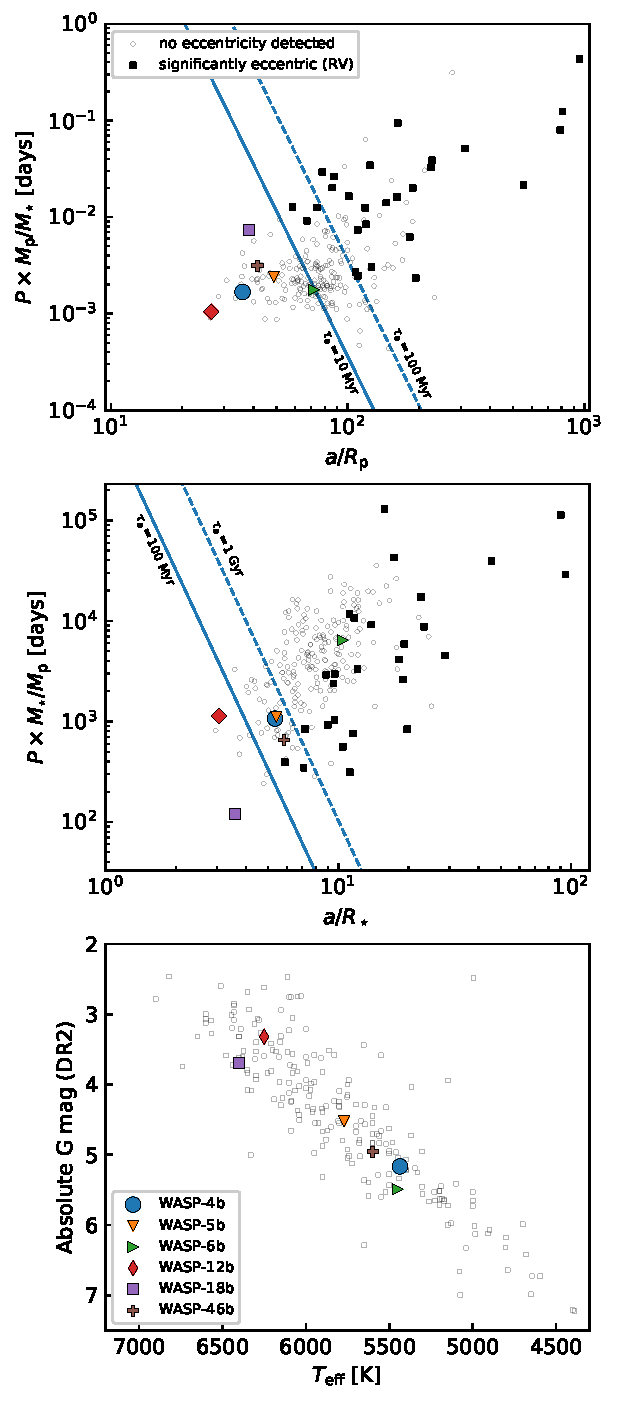
\includegraphics[width=0.48\textwidth]{f5.pdf}
	\end{center}
  \vspace{-0.5cm}
	\caption{
		{\bf Pecise long-term monitoring past 2025 will likely be needed to
	    understand WASP-4b.}
		Dots are as in Figure~\ref{fig:times}.
		Lines are 100 random draws from the posteriors of the apsidal
		precession model (orange), and the orbital decay model (blue).    
		\label{fig:future}
	}
\end{figure}

If TESS continues observing after its primary mission, it will observe
additional transits of WASP-4b in the early 2020s
(Figure~\ref{fig:future}).  High-precision ground-based transit
measurements could also be useful.  In order to rule between orbital
decay and apsidal precession, occultation measurements in both the
near term and also in the mid-2020s will be needed.  Additionally,
confirmation and extension of the linear RV trend suggested by
\citet{knutson_friends_2014} would help in understanding whether an
exterior companion in the system might explain any residual
eccentricity.  These observations should be carried out because they
will lead to new knowledge; either a measure of the stellar tidal
dissipation efficiency, or the eccentricity and Love number of the
planet.  Either outcome for a single system would be somewhat
interesting.  In the coming decade, wide-field photometric surveys
(TESS, HATPI, NGTS, PLATO) might even enable such measurements at a
population level, which would be extremely interesting.


\acknowledgements{
L.G.B.\ gladly acknowledges helpful discussions with
A.~Bailey, F.~Dai and V.~Van Eylen, and is grateful to the
people who have turned TESS from an idea into reality.
%
WASP-4 was included on the ``short-cadence'' target list thanks to the
Guest Investigator programs of J.\ Southworth and S.\ Kane (G011112
and G011183 respectively). 
%
This paper includes data collected by the TESS mission, which are
publicly available from the Mikulski Archive for Space Telescopes
(MAST).
%
Funding for the TESS mission is provided by NASA's Science Mission
directorate.
%
This research has made use of the NASA Exoplanet Archive, which is
operated by the California Institute of Technology, under contract
with the National Aeronautics and Space Administration under the
Exoplanet Exploration Program.
%
This work made use of NASA's Astrophysics Data System Bibliographic
Services.
%
This research has made use of the VizieR catalogue access tool, CDS,
Strasbourg, France. The original description of the VizieR service was
published in A\&AS 143, 23.
%
This work has made use of data from the European Space Agency (ESA)
mission {\it Gaia} (\url{https://www.cosmos.esa.int/gaia}), processed
by the {\it Gaia} Data Processing and Analysis Consortium (DPAC,
\url{https://www.cosmos.esa.int/web/gaia/dpac/consortium}). Funding
for the DPAC has been provided by national institutions, in particular
the institutions participating in the {\it Gaia} Multilateral
Agreement.
%
\newline
%
\facility{
	TESS \citep{ricker_transiting_2015},
	Gaia \citep{gaia_collaboration_gaia_2016,gaia_collaboration_gaia_2018}}
}
%
\software{
  \texttt{astrobase} \citep{bhatti_astrobase_2018},
  \texttt{astropy} \citep{the_astropy_collaboration_astropy_2018},
  \texttt{astroquery} \citep{astroquery_2018},
  \texttt{BATMAN} \citep{kreidberg_batman_2015},
  \texttt{corner} \citep{corner_2016},
  \texttt{emcee} \citep{foreman-mackey_emcee_2013},
  \texttt{IPython} \citep{perez_2007},
  \texttt{matplotlib} \citep{hunter_matplotlib_2007}, 
  \texttt{numpy} \citep{walt_numpy_2011}, 
  \texttt{pandas} \citep{mckinney-proc-scipy-2010},
  \texttt{scikit-learn} \citep{scikit-learn},
  \texttt{scipy} \citep{jones_scipy_2001}.
  }



%\clearpage

%\newpage
%% \begin{deluxetable}{} command tell LaTeX how many columns
%% there are and how to align them.
\startlongtable
\begin{deluxetable}{ccccc}
    
%% Keep a portrait orientation

%% Over-ride the default font size
%% Use Default (12pt)
\tabletypesize{\scriptsize}

%% Use \tablewidth{?pt} to over-ride the default table width.
%% If you are unhappy with the default look at the end of the
%% *.log file to see what the default was set at before adjusting
%% this value.

%% This is the title of the table.
\tablecaption{WASP-4b transit times, uncertainties, and references.}
\label{tab:transit_times}

%% This command over-rides LaTeX's natural table count
%% and replaces it with this number.  LaTeX will increment 
%% all other tables after this table based on this number
\tablenum{1}

%% The \tablehead gives provides the column headers.  It
%% is currently set up so that the column labels are on the
%% top line and the units surrounded by ()s are in the 
%% bottom line.  You may add more header information by writing
%% another line between these lines. For each column that requries
%% extra information be sure to include a \colhead{text} command
%% and remember to end any extra lines with \\ and include the 
%% correct number of &s.
\tablehead{
  \colhead{$t_{\rm tra}$ [BJD$_\mathrm{TDB}$]} &
  \colhead{$\sigma_{t_{\rm tra}}$ [days]} &
  \colhead{Epoch} & 
  \colhead{H13?} & 
  \colhead{Reference}
}

%% All data must appear between the \startdata and \enddata commands
% XXX pasted in from selected_transit_times.tex
\startdata
 2454368.59279 &      0.00033 &   -1059 &       1 &           \citet{wilson_wasp-4b_2008} \\
 2454396.69576 &      0.00012 &   -1038 &       1 &          \citet{gillon_improved_2009} \\
 2454697.79817 &      0.00009 &    -813 &       1 &             \citet{winn_transit_2009} \\
 2454701.81280 &      0.00022 &    -810 &       1 &             \citet{hoyer_tramos_2013} \\
 2454701.81303 &      0.00018 &    -810 &       1 &             \citet{hoyer_tramos_2013} \\
 2454705.82715 &      0.00029 &    -807 &       1 &             \citet{hoyer_tramos_2013} \\
 2454728.57767 &      0.00042 &    -790 &       1 &             \citet{hoyer_tramos_2013} \\
 2454732.59197 &      0.00050 &    -787 &       1 &             \citet{hoyer_tramos_2013} \\
 2454740.62125 &      0.00035 &    -781 &       1 &             \citet{hoyer_tramos_2013} \\
 2454748.65111 &      0.00007 &    -775 &       1 &             \citet{winn_transit_2009} \\
 2454752.66576 &      0.00069 &    -772 &       1 &           \citet{dragomir_terms_2011} \\
 2455041.72377 &      0.00018 &    -556 &       1 &             \citet{hoyer_tramos_2013} \\
 2455045.73853 &      0.00008 &    -553 &       1 &  \citet{sanchis-ojeda_starspots_2011} \\
 2455049.75325 &      0.00007 &    -550 &       1 &  \citet{sanchis-ojeda_starspots_2011} \\
 2455053.76774 &      0.00009 &    -547 &       1 &  \citet{sanchis-ojeda_starspots_2011} \\
 2455069.82661 &      0.00029 &    -535 &       1 &          \citet{nikolov_wasp-4b_2012} \\
 2455069.82670 &      0.00028 &    -535 &       1 &          \citet{nikolov_wasp-4b_2012} \\
 2455069.82617 &      0.00038 &    -535 &       1 &          \citet{nikolov_wasp-4b_2012} \\
 2455069.82676 &      0.00031 &    -535 &       1 &          \citet{nikolov_wasp-4b_2012} \\
 2455073.84128 &      0.00026 &    -532 &       1 &          \citet{nikolov_wasp-4b_2012} \\
 2455073.84108 &      0.00029 &    -532 &       1 &          \citet{nikolov_wasp-4b_2012} \\
 2455073.84111 &      0.00023 &    -532 &       1 &          \citet{nikolov_wasp-4b_2012} \\
 2455073.84114 &      0.00018 &    -532 &       1 &          \citet{nikolov_wasp-4b_2012} \\
 2455096.59148 &      0.00022 &    -515 &       1 &             \citet{hoyer_tramos_2013} \\
 2455100.60595 &      0.00012 &    -512 &       1 &  \citet{sanchis-ojeda_starspots_2011} \\
 2455112.64986 &      0.00039 &    -503 &       1 &          \citet{nikolov_wasp-4b_2012} \\
 2455112.65009 &      0.00033 &    -503 &       1 &          \citet{nikolov_wasp-4b_2012} \\
 2455112.65005 &      0.00031 &    -503 &       1 &          \citet{nikolov_wasp-4b_2012} \\
 2455112.65005 &      0.00049 &    -503 &       1 &          \citet{nikolov_wasp-4b_2012} \\
 2455132.72310 &      0.00041 &    -488 &       1 &             \citet{hoyer_tramos_2013} \\
 2455468.61943 &      0.00046 &    -237 &       1 &             \citet{hoyer_tramos_2013} \\
 2455526.16356 &      0.00008 &    -194 &       0 &       \citet{ranjan_atmospheric_2014} \\
 2455828.60375 &      0.00041 &      32 &       1 &             \citet{hoyer_tramos_2013} \\
 2455832.61815 &      0.00041 &      35 &       1 &             \citet{hoyer_tramos_2013} \\
 2455844.66287 &      0.00009 &      44 &       0 &           \citet{huitson_gemini_2017} \\
 2456216.69123 &      0.00006 &     322 &       0 &           \citet{huitson_gemini_2017} \\
 2456576.67556 &      0.00005 &     591 &       0 &           \citet{huitson_gemini_2017} \\
 2456924.61561 &      0.00006 &     851 &       0 &           \citet{huitson_gemini_2017} \\
 2458355.18490 &      0.00024 &    1920 &       0 &                             This work \\
 2458356.52251 &      0.00026 &    1921 &       0 &                             This work \\
 2458357.86101 &      0.00024 &    1922 &       0 &                             This work \\
 2458359.19951 &      0.00025 &    1923 &       0 &                             This work \\
 2458360.53708 &      0.00027 &    1924 &       0 &                             This work \\
 2458361.87539 &      0.00024 &    1925 &       0 &                             This work \\
 2458363.21412 &      0.00027 &    1926 &       0 &                             This work \\
 2458364.55192 &      0.00025 &    1927 &       0 &                             This work \\
 2458365.89064 &      0.00026 &    1928 &       0 &                             This work \\
 2458369.90503 &      0.00027 &    1931 &       0 &                             This work \\
 2458371.24297 &      0.00026 &    1932 &       0 &                             This work \\
 2458372.58136 &      0.00027 &    1933 &       0 &                             This work \\
 2458373.91982 &      0.00027 &    1934 &       0 &                             This work \\
 2458375.25801 &      0.00024 &    1935 &       0 &                             This work \\
 2458376.59621 &      0.00024 &    1936 &       0 &                             This work \\
 2458377.93443 &      0.00026 &    1937 &       0 &                             This work \\
 2458379.27317 &      0.00026 &    1938 &       0 &                             This work \\
 2458380.61097 &      0.00027 &    1939 &       0 &                             This work \\
\enddata

%% Include any \tablenotetext{key}{text}, \tablerefs{ref list},
%% or \tablecomments{text} between the \enddata and 
%% \end{deluxetable} commands

%% General table comment marker
\tablecomments{
    $t_{\rm tra}$ is the measured transit midtime, and $\sigma_{t_{\rm
    tra}}$ is its $1\sigma$ uncertainty.
    $\sigma_{t_0}$ was evaluated from the sampled posteriors by taking
    the maximum of the difference between the 84th percentile
    minus the median, and the median minus the 16th percentile.
    The ``Reference'' column refers to the work describing the
    original observations.
    The ``H13?'' column is 1 if the mid-time value was taken from 
    \citet{hoyer_tramos_2013}.  Otherwise, the mid-time
    came from the column listed in ``Reference''.
    The \citet{hoyer_tramos_2013} BJD$_{\rm TT}$ times are equal to
    BJD$_{\rm TDB}$ for our purposes \citep{urban_explanatory_2012}.
    We omitted the timing measurements from
    \citet{southworth_high-precision_2009}, since there were technical
    problems with the computer clock at the time of
    observation~\citep{nikolov_wasp-4b_2012}.
}
\end{deluxetable}


%\clearpage
%\newpage
%% \begin{deluxetable}{} command tell LaTeX how many columns
%% there are and how to align them.
\startlongtable
\begin{deluxetable}{cccc}
    
%% Keep a portrait orientation

%% Over-ride the default font size
%% Use Default (12pt)
\tabletypesize{\footnotesize}

%% Use \tablewidth{?pt} to over-ride the default table width.
%% If you are unhappy with the default look at the end of the
%% *.log file to see what the default was set at before adjusting
%% this value.

%% This is the title of the table.
\tablecaption{WASP-4b occultation times, uncertainties, and references.}
\label{tab:occultation_times}

%% This command over-rides LaTeX's natural table count
%% and replaces it with this number.  LaTeX will increment 
%% all other tables after this table based on this number
\tablenum{3}

%% The \tablehead gives provides the column headers.  It
%% is currently set up so that the column labels are on the
%% top line and the units surrounded by ()s are in the 
%% bottom line.  You may add more header information by writing
%% another line between these lines. For each column that requries
%% extra information be sure to include a \colhead{text} command
%% and remember to end any extra lines with \\ and include the 
%% correct number of &s.
\tablehead{
  \colhead{$t_{\rm occ}$ [BJD$_\mathrm{TDB}$]} &
  \colhead{$\sigma_{t_{\rm occ}}$ [days]} &
  \colhead{Epoch} & 
  \colhead{Reference}
}

%% All data must appear between the \startdata and \enddata commands
% XXX pasted in from selected_transit_times.tex
\startdata
 2455102.61210 &      0.00109 &    -511 &  \citet{caceres_ground-based_2011}\tablenotemark{a} \\
 2455172.20159 &      0.00130 &    -459 &      \citet{beerer_secondary_2011} \\
 2455174.87780 &      0.00087 &    -457 &      \citet{beerer_secondary_2011} \\
 2456907.88714 &      0.00290 &     838 &        \citet{zhou_secondary_2015}\tablenotemark{b} \\
\enddata

%% Include any \tablenotetext{key}{text}, \tablerefs{ref list},
%% or \tablecomments{text} between the \enddata and 
%% \end{deluxetable} commands

%% General table comment marker
\tablecomments{
	$t_{\rm occ}$ is the measured occultation midtime, minus the
	$2a/c=22.8$ second light travel time;
	$\sigma_{t_{\rm occ}}$ is the $1\sigma$ uncertainty on the occultation
	time.
}
\tablenotetext{a}{
\citet{caceres_ground-based_2011} reported this time in ``HJD'', with
an unspecified time standard. We assumed the time was originally in
${\rm HJD}_{\rm UTC}$, inflated the uncertainties by 69.184 seconds,
and converted to ${\rm BJD}_{\rm TDB}$ for the time reported.
}
\tablenotetext{b}{
\citet{zhou_secondary_2015} fixed the epoch, and let $e\cos\omega$
float. Using the reported dates of observation, we converted their
$e\cos\omega$ values into an occultation time using
Equation~\ref{eq:occultation_time} of the text. 
}

\end{deluxetable}


%\clearpage
%\newpage
%\renewcommand{\arraystretch}{1.0}

\startlongtable
\begin{deluxetable}{lc}

\tabletypesize{\footnotesize}

\tablenum{4}

%\tablewidth{0pt}

\tablecaption{Best-fit model parameters.}
\label{tab:bestfit}

\tablehead{
  \colhead{Parameter} &
  \colhead{Median Value~(Unc.)\tablenotemark{a}}
}

\startdata
~~~~~~{\it Constant period} &  \\
$t_0$\,[${\rm BJD}_{\rm TBD}$]    & 2455804.515752(+19)(-19)              \\
$P$\,[days]                       & 1.338231466(+23)(-22)                 \\
~~~~~~{\it Constant period derivative} &  \\
$t_0$~[${\rm BJD}_{\rm TBD}$]     & 2455804.515918(+24)(-24)              \\
$P$\,[days]                       & 1.338231679(+31)(-31)                 \\
$dP/dt$                           & $-4.00(+37)(-38) \times 10^{-10}$     \\
~~~~~~{\it Apsidal precession} &  \\
$t_0$~[${\rm BJD}_{\rm TBD}$]     & 2455804.51530(+25)(-31)               \\
$P_{\rm s}$\,[days]               & 1.33823127(+20)(-48)                  \\
$e$                               & $1.92^{+1.93}_{-0.76} \times 10^{-3}$ \\
$\omega_0$\,[rad]                 & 2.40(+38)(-34)                        \\
$d\omega/dE$~[rad\,epoch$^{-1}$]  & $8.70^{+3.01}_{-2.30} \times 10^{-4}$ \\
\enddata
\tablenotetext{a}{
The numbers in parenthesis give the $68\%$ confidence interval for the final
two digits, where appropriate.
}
\end{deluxetable}



\bibliographystyle{yahapj}                            
\bibliography{bibliography} 

%\clearpage
%\newpage

\appendix

\section{Verifying the TESS Time Stamps}
\label{sec:verify_tess}

Any systematic offset between the TESS times and the true barycentric
reference would cast doubt on the results of this study.  There is
historic precedent: Kepler had a systematic error in its timestamps
that was corrected only in Q14~\citep[][Section
3.4]{kepler_DR19_2013}.

We devised two checks on the absolute calibration of the TESS time
system.  First, in \S~\ref{sec:headers}, we recalculate and confirm
the barycentric correction reported by SPOC in the TESS lightcurve
file headers.  In \S~\ref{sec:hj_verification}, we measure the transit
times of other hot Jupiters, and use them to rule out a global TESS
time offset larger than about a minute.  The latter test confirms that
WASP-4b is an outlier.

\subsection{Using the headers of the lightcurve files}
\label{sec:headers}

The TESS lightcurve files provide observation start and end times in
three different time systems: ${\rm JD}_{\rm UTC}$, ${\rm JD}_{\rm
TDB}$, and ${\rm BJD}_{\rm TDB}$.  First, we verified for a few select
lightcurve files that ${\rm JD}_{\rm UTC}$ lagged behind ${\rm
JD}_{\rm TDB}$ by the expected $32.184 + N\,{\rm seconds}$, where $N$
is the number of leap-seconds since 1961. For the relevant observation
time, $N=37$, and the offset was as expected.  Then, using the ${\rm
JD}_{\rm UTC}$ timestamp, we recalculated the barycentric correction
computed by SPOC, using the \citealt{eastman_achieving_2010}
calculator.  Due to the first author's ignorance of the spacecraft
position, we assumed that the observer was located at the Earth's
geocenter, and used the correct direction for each star.  This gave us
times in ${\rm BJD}_{\rm TDB}$ that agreed with the archival times to
within 1.7 seconds.  This offset is comparable to the light-travel
delay expected for TESS on its orbit from perigee of $\approx
20R_\oplus$ to apogee of $\approx 60R_\oplus$.

This calculation bounds any error in the SPOC barycentric julian date
correction to be less than 1.7 seconds.  This is smaller than the
effect of interest, so we treat the SPOC BJD correction as
``verified'', and proceed to a subsequent test.


\subsection{Using other hot Jupiters as references}
\label{sec:hj_verification}

\begin{figure*}[ht!]
  \begin{center}
    \leavevmode
    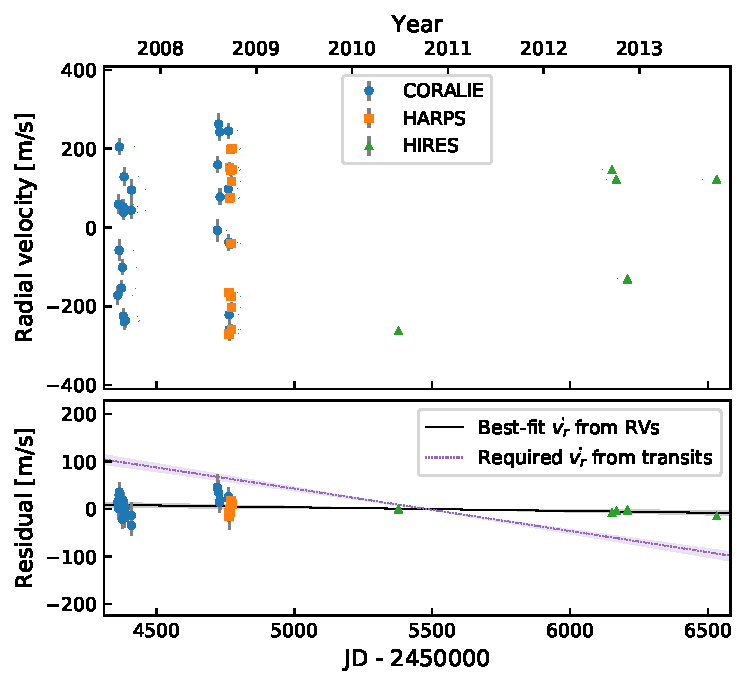
\includegraphics[width=0.9\textwidth]{f6.pdf}
  \end{center}
  \vspace{-0.5cm}
  \caption{
    {\bf There is no evidence for a systematic offset between TESS
    times and the barycentric reference.}
    While the WASP-4b transits fell about 75 seconds earlier than
    predicted, other well-observed hot Jupiters, in particular WASP-6b
    and WASP-18b, arrived on time.  Ticks are observed TESS transit
    midtimes; the blue distribution function is a kernel density
    estimate; the orange distribution function is a gaussian centered
    on zero using the indicated $1\sigma$ standard deviation in the
    prediction
    ($\sigma_{\rm predicted}$).
    \label{fig:hjs}
  }
\end{figure*}

If the observed timing delay in WASP-4b were caused by a systematic
offset between the TESS times and the ${\rm
BJD}_{\rm TDB}$ reference, we might expect that it would apply to
other hot Jupiters as well.  This test can rule out an important class
of clock error~--~a systematic global offset.

To explore this possibility, we repeat the timing analysis of the main
paper, for other hot Jupiters with long preceding observing baselines.
We first checked which hot Jupiters were observed over the first two
TESS sectors using a combination of
\texttt{tessmaps}\footnote{\url{github.com/lgbouma/tessmaps}} and
TEPCat \citep{southworth_homogeneous_2011}.  We then selected hot
Jupiters for which there were at least five distinct epochs reported
in the peer-reviewed literature.  We required that each observation be
of a single transit, that the midpoint be fit as a free parameter, and
that the time system be clearly documented.  Our final hot Jupiter
sample included WASPs-4b, -5b, -6b, -18b, and -46b.  The collected and
measured times are given in Tables~5, 6, 7, and 8 for each.

Using the literature timing data for each hot Jupiter, we then
performed a least-squares fit to a linear ephemeris.  Using the
best-fit values and variances, we calculated the uncertainty on the
predicted transit time during the TESS observations.  This gave 9, 94,
18, 42, and 60 seconds for WASPs-4b, -5b, -6b, -18b, and -46b.  We
show in Figure~\ref{fig:hjs} that WASP-4b is the only hot Jupiter that
transited significantly earlier than expected.

To convert this intuition into a quantitative limit, for each hot
Jupiter we considered the model
\begin{equation}
  t_{\rm tra}(E) = t_0 + PE + t_{\rm offset},
\end{equation}
for $t_{\rm offset}$ a systematic constant offset between the reported
timestamps and the true ${\rm BJD}_{\rm TDB}$ reference.  Our priors
were
\begin{align}
  t_0 &\sim \mathcal{N}[t_0', \sigma_{t_0'}], \\
  P &\sim \mathcal{N}[P', \sigma_{P'}], \\
  t_{\rm offset} &\sim \mathcal{U}[-20\sigma_{t_0'},20\sigma_{t_0'}],
\end{align}
where $\mathcal{N}$ and $\mathcal{U}$ denote a normal and uniform
distribution, $(t_0', P')$ are the best-fit reference time and period
using only the literature transit times, and $(\sigma_{t_0'},
\sigma_{P'})$ are their uncertainties.

For each planet, we then ask: what fraction of the posterior for
$t_{\rm offset}$ is consistent with an offset worse than $77$ seconds?
For WASP-4b, the answer is unsurpringly about half.  For WASP-6b, the
most constraining object, about 1 sample in 2 million is consistent
with such a timing offset ($4.9\sigma$).  For WASP-18b, 1 in 63
samples would be consistent with this timing offset ($2.1\sigma$), and
in WASP-46b, the limit is 1 in 38 samples ($1.9\sigma$).  For WASP-5b,
the predicted time is too imprecise to rule out timing offsets at the
necessary amplitude.  Multiplying the three independent probabilities
for WASPs-5b, 6b, and -18b, we rule out $t_{\rm offset} < -77\ {\rm
seconds}$ at $6.3\sigma$, or about about 1 part in 5 billion.


%\clearpage
%\newpage
%% \begin{deluxetable}{} command tell LaTeX how many columns
%% there are and how to align them.
\startlongtable
\begin{deluxetable}{ccccc}
    
%% Keep a portrait orientation

%% Over-ride the default font size
%% Use Default (12pt)
\tabletypesize{\scriptsize}

%% Use \tablewidth{?pt} to over-ride the default table width.
%% If you are unhappy with the default look at the end of the
%% *.log file to see what the default was set at before adjusting
%% this value.

%% This is the title of the table.
\tablecaption{WASP-5b transit times, uncertainties, and references.}
\label{tab:WASP-5b}

%% This command over-rides LaTeX's natural table count
%% and replaces it with this number.  LaTeX will increment 
%% all other tables after this table based on this number
\tablenum{4}

%% The \tablehead gives provides the column headers.  It
%% is currently set up so that the column labels are on the
%% top line and the units surrounded by ()s are in the 
%% bottom line.  You may add more header information by writing
%% another line between these lines. For each column that requries
%% extra information be sure to include a \colhead{text} command
%% and remember to end any extra lines with \\ and include the 
%% correct number of &s.
\tablehead{
  \colhead{$t_{\rm tra}$ [BJD$_\mathrm{TDB}$]} &
  \colhead{$\sigma_{t_{\rm tra}}$ [days]} &
  \colhead{Epoch} & 
  \colhead{Reference}
}

%% All data must appear between the \startdata and \enddata commands
\startdata
 2454383.76750 &      0.00040 &    -885 &           \citet{anderson_wasp-5b_2008} \\
 2454387.02275 &      0.00100 &    -883 &           \citet{anderson_wasp-5b_2008} \\
 2454636.17459 &      0.00082 &    -730 &         \citet{fukui_measurements_2011} \\
 2454699.68303 &      0.00041 &    -691 &              \citet{hoyer_transit_2012} \\
 2454707.82465 &      0.00052 &    -686 &              \citet{hoyer_transit_2012} \\
 2454707.82523 &      0.00025 &    -686 &  \citet{southworth_high-precision_2009} \\
 2454730.62243 &      0.00031 &    -672 &  \citet{southworth_high-precision_2009} \\
 2454730.62301 &      0.00076 &    -672 &              \citet{hoyer_transit_2012} \\
 2454761.56356 &      0.00047 &    -653 &              \citet{hoyer_transit_2012} \\
 2454772.96212 &      0.00075 &    -646 &         \citet{fukui_measurements_2011} \\
 2454774.59093 &      0.00030 &    -645 &              \citet{hoyer_transit_2012} \\
 2454787.61792 &      0.00069 &    -637 &              \citet{hoyer_transit_2012} \\
 2455005.82714 &      0.00036 &    -503 &              \citet{hoyer_transit_2012} \\
 2455049.79540 &      0.00080 &    -476 &              \citet{hoyer_transit_2012} \\
 2455075.84947 &      0.00056 &    -460 &             \citet{dragomir_terms_2011} \\
 2455079.10830 &      0.00079 &    -458 &         \citet{fukui_measurements_2011} \\
 2455110.04607 &      0.00089 &    -439 &         \citet{fukui_measurements_2011} \\
 2455123.07611 &      0.00079 &    -431 &         \citet{fukui_measurements_2011} \\
 2455129.58759 &      0.00043 &    -427 &              \citet{hoyer_transit_2012} \\
 2455364.08150 &      0.00110 &    -283 &         \citet{fukui_measurements_2011} \\
 2455377.10955 &      0.00093 &    -275 &         \citet{fukui_measurements_2011} \\
 2455448.75927 &      0.00110 &    -231 &             \citet{dragomir_terms_2011} \\
 2456150.61479 &      0.00056 &     200 &          \citet{moyano_multi-band_2017} \\
 2456150.61396 &      0.00057 &     200 &          \citet{moyano_multi-band_2017} \\
 2458355.50829 &      0.00083 &    1554 &                               This work \\
 2458357.13741 &      0.00071 &    1555 &                               This work \\
 2458358.76412 &      0.00068 &    1556 &                               This work \\
 2458360.39377 &      0.00070 &    1557 &                               This work \\
 2458362.02273 &      0.00073 &    1558 &                               This work \\
 2458363.64908 &      0.00090 &    1559 &                               This work \\
 2458365.27827 &      0.00071 &    1560 &                               This work \\
 2458366.90627 &      0.00075 &    1561 &                               This work \\
 2458370.16411 &      0.00076 &    1563 &                               This work \\
 2458371.79126 &      0.00071 &    1564 &                               This work \\
 2458373.42123 &      0.00075 &    1565 &                               This work \\
 2458375.04910 &      0.00069 &    1566 &                               This work \\
 2458376.67856 &      0.00074 &    1567 &                               This work \\
 2458378.30530 &      0.00087 &    1568 &                               This work \\
 2458379.93419 &      0.00082 &    1569 &                               This work \\
\enddata

%% Include any \tablenotetext{key}{text}, \tablerefs{ref list},
%% or \tablecomments{text} between the \enddata and 
%% \end{deluxetable} commands

%% General table comment marker
\tablecomments{
    $t_{\rm tra}$ is the measured transit midtime, and $\sigma_{t_{\rm tra}}$ is its
    $1\sigma$ uncertainty.
    The ``Reference'' column refers to the work describing the
    original observations.
    All the literature times except for the two \citet{moyano_multi-band_2017}
    times are from the homogeneous \citet{hoyer_transit_2012} analysis.
}

\end{deluxetable}

%% \begin{deluxetable}{} command tell LaTeX how many columns
%% there are and how to align them.
\startlongtable
\begin{deluxetable}{ccccc}
    
%% Keep a portrait orientation

%% Over-ride the default font size
%% Use Default (12pt)
\tabletypesize{\scriptsize}
%% Use \tablewidth{?pt} to over-ride the default table width.
%% If you are unhappy with the default look at the end of the
%% *.log file to see what the default was set at before adjusting
%% this value.

%% This is the title of the table.
\tablecaption{WASP-6b transit times, uncertainties, and references.}
\label{tab:WASP-6b}

%% This command over-rides LaTeX's natural table count
%% and replaces it with this number.  LaTeX will increment 
%% all other tables after this table based on this number
\tablenum{6}

%% The \tablehead gives provides the column headers.  It
%% is currently set up so that the column labels are on the
%% top line and the units surrounded by ()s are in the 
%% bottom line.  You may add more header information by writing
%% another line between these lines. For each column that requries
%% extra information be sure to include a \colhead{text} command
%% and remember to end any extra lines with \\ and include the 
%% correct number of &s.
\tablehead{
  \colhead{$t_{\rm tra}$ [BJD$_\mathrm{TDB}$]} &
  \colhead{$\sigma_{t_{\rm tra}}$ [days]} &
  \colhead{Epoch} & 
  \colhead{Reference}
}

%% All data must appear between the \startdata and \enddata commands
\startdata
 2454425.02167 &      0.00022 &    -398 &        \citet{gillon_discovery_2009} \\
 2455009.83622 &      0.00021 &    -224 &  \citet{tregloan-reed_transits_2015} \\
 2455046.80720 &      0.00015 &    -213 &  \citet{tregloan-reed_transits_2015} \\
 2455073.69529 &      0.00013 &    -205 &  \citet{tregloan-reed_transits_2015} \\
 2455409.79541 &      0.00010 &    -105 &  \citet{tregloan-reed_transits_2015} \\
 2455446.76621 &      0.00058 &     -94 &          \citet{dragomir_terms_2011} \\
 2455473.65439 &      0.00097 &     -86 &     \citet{jordan_ground-based_2013} \\
 2455846.72540 &      0.00045 &      25 &         \citet{sada_extrasolar_2012} \\
 2456088.71801 &      0.00013 &      97 &             \citet{nikolov_hst_2015} \\
 2456095.43974 &      0.00017 &      99 &             \citet{nikolov_hst_2015} \\
 2456132.41082 &      0.00017 &     110 &             \citet{nikolov_hst_2015} \\
 2458357.39410 &      0.00033 &     772 &                            This work \\
 2458360.75573 &      0.00033 &     773 &                            This work \\
 2458364.11691 &      0.00032 &     774 &                            This work \\
 2458370.83872 &      0.00033 &     776 &                            This work \\
 2458374.19952 &      0.00031 &     777 &                            This work \\
 2458377.56026 &      0.00033 &     778 &                            This work \\
 2458380.92185 &      0.00038 &     779 &                            This work \\
\enddata

%% Include any \tablenotetext{key}{text}, \tablerefs{ref list},
%% or \tablecomments{text} between the \enddata and 
%% \end{deluxetable} commands

%% General table comment marker
\tablecomments{
    $t_{\rm tra}$ is the measured transit midtime, and $\sigma_{t_{\rm tra}}$ is its
    $1\sigma$ uncertainty.
    The ``Reference'' column refers to the work describing the
    original observations.
}

\end{deluxetable}

%% \begin{deluxetable}{} command tell LaTeX how many columns
%% there are and how to align them.
\startlongtable
\begin{deluxetable}{ccccc}
    
%% Keep a portrait orientation

%% Over-ride the default font size
%% Use Default (12pt)
\tabletypesize{\scriptsize}
%% Use \tablewidth{?pt} to over-ride the default table width.
%% If you are unhappy with the default look at the end of the
%% *.log file to see what the default was set at before adjusting
%% this value.

%% This is the title of the table.
\tablecaption{WASP-18b transit times, uncertainties, and references.}
\label{tab:WASP-18b}

%% This command over-rides LaTeX's natural table count
%% and replaces it with this number.  LaTeX will increment 
%% all other tables after this table based on this number
\tablenum{7}

%% The \tablehead gives provides the column headers.  It
%% is currently set up so that the column labels are on the
%% top line and the units surrounded by ()s are in the 
%% bottom line.  You may add more header information by writing
%% another line between these lines. For each column that requries
%% extra information be sure to include a \colhead{text} command
%% and remember to end any extra lines with \\ and include the 
%% correct number of &s.
\tablehead{
  \colhead{$t_{\rm tra}$ [BJD$_\mathrm{TDB}$]} &
  \colhead{$\sigma_{t_{\rm tra}}$ [days]} &
  \colhead{Epoch} & 
  \colhead{Reference}
}

%% All data must appear between the \startdata and \enddata commands
\startdata
 2454221.48163 &      0.00038 &   -3730 &    \citet{hellier_orbital_2009} \\
 2455221.30420 &      0.00010 &   -2668 &     \citet{maxted_spitzer_2013} \\
 2455432.18970 &      0.00010 &   -2444 &     \citet{maxted_spitzer_2013} \\
 2455470.78850 &      0.00040 &   -2403 &     \citet{maxted_spitzer_2013} \\
 2455473.61440 &      0.00090 &   -2400 &     \citet{maxted_spitzer_2013} \\
 2455554.57860 &      0.00050 &   -2314 &     \citet{maxted_spitzer_2013} \\
 2455570.58400 &      0.00048 &   -2297 &     \citet{maxted_spitzer_2013} \\
 2455876.55590 &      0.00130 &   -1972 &     \citet{maxted_spitzer_2013} \\
 2456896.14780 &      0.00080 &    -889 &  \citet{wilkins_searching_2017} \\
 2457255.78320 &      0.00030 &    -507 &  \citet{wilkins_searching_2017} \\
 2457319.80100 &      0.00039 &    -439 &  \citet{wilkins_searching_2017} \\
 2458354.45778 &      0.00015 &     660 &                       This work \\
 2458355.39934 &      0.00015 &     661 &                       This work \\
 2458356.34073 &      0.00016 &     662 &                       This work \\
 2458357.28228 &      0.00017 &     663 &                       This work \\
 2458358.22348 &      0.00017 &     664 &                       This work \\
 2458359.16512 &      0.00016 &     665 &                       This work \\
 2458360.10662 &      0.00016 &     666 &                       This work \\
 2458361.04813 &      0.00017 &     667 &                       This work \\
 2458361.98968 &      0.00016 &     668 &                       This work \\
 2458362.93129 &      0.00016 &     669 &                       This work \\
 2458363.87266 &      0.00018 &     670 &                       This work \\
 2458364.81373 &      0.00016 &     671 &                       This work \\
 2458365.75526 &      0.00017 &     672 &                       This work \\
 2458366.69704 &      0.00019 &     673 &                       This work \\
 2458367.63835 &      0.00187 &     674 &                       This work \\
 2458369.52126 &      0.00017 &     676 &                       This work \\
 2458370.46285 &      0.00017 &     677 &                       This work \\
 2458371.40405 &      0.00016 &     678 &                       This work \\
 2458372.34536 &      0.00017 &     679 &                       This work \\
 2458373.28727 &      0.00017 &     680 &                       This work \\
 2458374.22817 &      0.00016 &     681 &                       This work \\
 2458375.16976 &      0.00016 &     682 &                       This work \\
 2458376.11124 &      0.00017 &     683 &                       This work \\
 2458377.05269 &      0.00016 &     684 &                       This work \\
 2458377.99448 &      0.00017 &     685 &                       This work \\
 2458378.93572 &      0.00016 &     686 &                       This work \\
 2458379.87720 &      0.00016 &     687 &                       This work \\
 2458380.81891 &      0.00017 &     688 &                       This work \\
\enddata

%% Include any \tablenotetext{key}{text}, \tablerefs{ref list},
%% or \tablecomments{text} between the \enddata and 
%% \end{deluxetable} commands

%% General table comment marker
\tablecomments{
    $t_{\rm tra}$ is the measured transit midtime, and $\sigma_{t_{\rm tra}}$ is its
    $1\sigma$ uncertainty.
    The ``Reference'' column refers to the work describing the
    original observations.
    All the literature times are from the homogeneous
    \citet{wilkins_searching_2017} analysis.
}

\end{deluxetable}

%% \begin{deluxetable}{} command tell LaTeX how many columns
%% there are and how to align them.
\startlongtable
\begin{deluxetable}{ccccc}
    
%% Keep a portrait orientation

%% Over-ride the default font size
%% Use Default (12pt)
\tabletypesize{\scriptsize}
%% Use \tablewidth{?pt} to over-ride the default table width.
%% If you are unhappy with the default look at the end of the
%% *.log file to see what the default was set at before adjusting
%% this value.

%% This is the title of the table.
\tablecaption{WASP-46b transit times, uncertainties, and references.}
\label{tab:WASP-46b}

%% This command over-rides LaTeX's natural table count
%% and replaces it with this number.  LaTeX will increment 
%% all other tables after this table based on this number
\tablenum{8}

%% The \tablehead gives provides the column headers.  It
%% is currently set up so that the column labels are on the
%% top line and the units surrounded by ()s are in the 
%% bottom line.  You may add more header information by writing
%% another line between these lines. For each column that requries
%% extra information be sure to include a \colhead{text} command
%% and remember to end any extra lines with \\ and include the 
%% correct number of &s.
\tablehead{
  \colhead{$t_{\rm tra}$ [BJD$_\mathrm{TDB}$]} &
  \colhead{$\sigma_{t_{\rm tra}}$ [days]} &
  \colhead{Epoch} & 
  \colhead{Reference}
}

%% All data must appear between the \startdata and \enddata commands
\startdata
 2455396.60785 &      0.00062 &    -673 &  \citet{anderson_wasp-44b_2012} \\
 2455449.53082 &      0.00026 &    -636 &  \citet{anderson_wasp-44b_2012} \\
 2455722.73178 &      0.00023 &    -445 &    \citet{ciceri_physical_2016} \\
 2455757.06195 &      0.00094 &    -421 &    \citet{petrucci_search_2018} \\
 2455858.61833 &      0.00009 &    -350 &    \citet{ciceri_physical_2016} \\
 2456108.92771 &      0.00094 &    -175 &    \citet{petrucci_search_2018} \\
 2456111.79422 &      0.00016 &    -173 &    \citet{ciceri_physical_2016} \\
 2456111.79413 &      0.00012 &    -173 &    \citet{ciceri_physical_2016} \\
 2456111.79424 &      0.00015 &    -173 &    \citet{ciceri_physical_2016} \\
 2456130.38895 &      0.00042 &    -160 &    \citet{petrucci_search_2018} \\
 2456131.81456 &      0.00112 &    -159 &    \citet{petrucci_search_2018} \\
 2456194.75916 &      0.00027 &    -115 &    \citet{ciceri_physical_2016} \\
 2456217.64127 &      0.00015 &     -99 &    \citet{ciceri_physical_2016} \\
 2456217.64156 &      0.00013 &     -99 &    \citet{ciceri_physical_2016} \\
 2456227.65574 &      0.00060 &     -92 &    \citet{petrucci_search_2018} \\
 2456407.88096 &      0.00015 &      34 &    \citet{ciceri_physical_2016} \\
 2456407.88085 &      0.00018 &      34 &    \citet{ciceri_physical_2016} \\
 2456407.88148 &      0.00028 &      34 &    \citet{ciceri_physical_2016} \\
 2456407.88159 &      0.00043 &      34 &    \citet{ciceri_physical_2016} \\
 2456460.80526 &      0.00017 &      71 &    \citet{ciceri_physical_2016} \\
 2456460.80450 &      0.00024 &      71 &    \citet{ciceri_physical_2016} \\
 2456460.80547 &      0.00064 &      71 &    \citet{ciceri_physical_2016} \\
 2456510.86818 &      0.00060 &     106 &    \citet{petrucci_search_2018} \\
 2456510.86699 &      0.00015 &     106 &    \citet{petrucci_search_2018} \\
 2456516.58667 &      0.00119 &     110 &    \citet{petrucci_search_2018} \\
 2456520.88012 &      0.00064 &     113 &    \citet{petrucci_search_2018} \\
 2456533.75260 &      0.00071 &     122 &    \citet{ciceri_physical_2016} \\
 2456533.75480 &      0.00015 &     122 &    \citet{ciceri_physical_2016} \\
 2456576.66289 &      0.00109 &     152 &    \citet{petrucci_search_2018} \\
 2456589.54197 &      0.00090 &     161 &    \citet{petrucci_search_2018} \\
 2456609.56653 &      0.00043 &     175 &    \citet{petrucci_search_2018} \\
 2456839.85440 &      0.00123 &     336 &    \citet{petrucci_search_2018} \\
 2456862.74085 &      0.00048 &     352 &    \citet{petrucci_search_2018} \\
 2456882.76566 &      0.00073 &     366 &    \citet{petrucci_search_2018} \\
 2456885.62429 &      0.00053 &     368 &    \citet{petrucci_search_2018} \\
 2456915.66040 &      0.00123 &     389 &    \citet{petrucci_search_2018} \\
 2456942.83880 &      0.00078 &     408 &    \citet{petrucci_search_2018} \\
 2456948.56384 &      0.00074 &     412 &    \citet{petrucci_search_2018} \\
 2457274.68458 &      0.00184 &     640 &    \citet{petrucci_search_2018} \\
 2457294.70886 &      0.00140 &     654 &    \citet{petrucci_search_2018} \\
 2457550.74797 &      0.00031 &     833 &    \citet{petrucci_search_2018} \\
 2457593.65692 &      0.00024 &     863 &    \citet{petrucci_search_2018} \\
 2457600.80985 &      0.00039 &     868 &    \citet{petrucci_search_2018} \\
 2457610.82286 &      0.00020 &     875 &    \citet{petrucci_search_2018} \\
 2458326.00972 &      0.00091 &    1375 &                       This work \\
 2458327.43899 &      0.00093 &    1376 &                       This work \\
 2458328.86970 &      0.00094 &    1377 &                       This work \\
 2458330.29965 &      0.00105 &    1378 &                       This work \\
 2458331.73234 &      0.00105 &    1379 &                       This work \\
 2458333.15977 &      0.00086 &    1380 &                       This work \\
 2458334.59230 &      0.00095 &    1381 &                       This work \\
 2458336.02222 &      0.00082 &    1382 &                       This work \\
 2458337.45111 &      0.00099 &    1383 &                       This work \\
 2458340.31143 &      0.00093 &    1385 &                       This work \\
 2458341.74347 &      0.00093 &    1386 &                       This work \\
 2458343.17362 &      0.00093 &    1387 &                       This work \\
 2458344.60303 &      0.00110 &    1388 &                       This work \\
 2458346.03436 &      0.00091 &    1389 &                       This work \\
 2458347.46335 &      0.00168 &    1390 &                       This work \\
 2458348.89621 &      0.00086 &    1391 &                       This work \\
 2458350.32672 &      0.00101 &    1392 &                       This work \\
 2458351.75486 &      0.00103 &    1393 &                       This work \\
\enddata

%% Include any \tablenotetext{key}{text}, \tablerefs{ref list},
%% or \tablecomments{text} between the \enddata and 
%% \end{deluxetable} commands

%% General table comment marker
\tablecomments{
    $t_{\rm tra}$ is the measured transit midtime, and $\sigma_{t_{\rm tra}}$ is its
    $1\sigma$ uncertainty.
    The ``Reference'' column refers to the work describing the
    original observations.
    All the literature times are from the homogeneous
    \citet{petrucci_search_2018} analysis. 14 of the lightcurves
    were acquired by ETD observers \citep[see][]{petrucci_search_2018}.
}

\end{deluxetable}





% \section{Verifying the WASP-4 Archival Times}
% \label{sec:verify_archival_times}
% 
% \begin{figure*}[ht!]
%   \begin{center}
%     \leavevmode
%     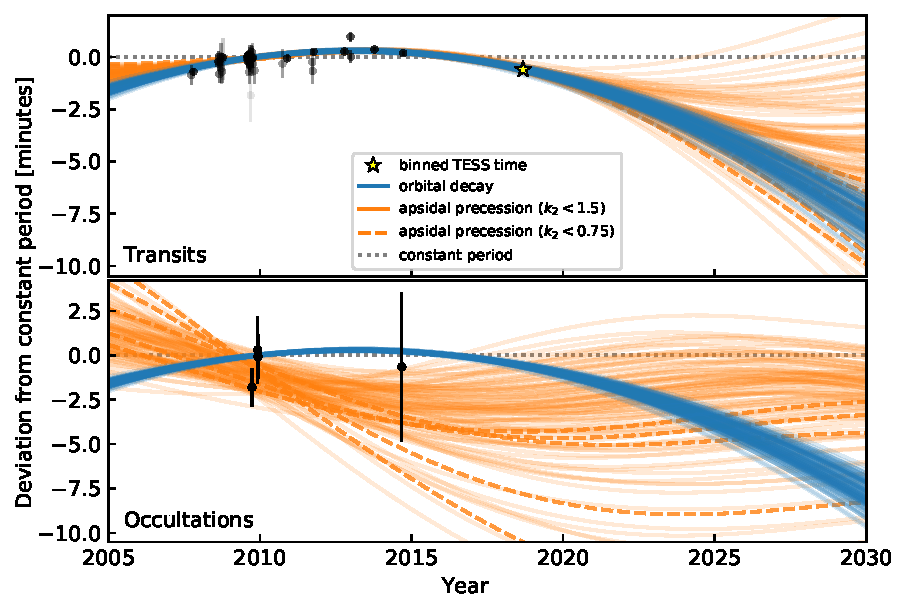
\includegraphics[width=0.9\textwidth]{f7.pdf}
%   \end{center}
%   \caption{
%     {\bf Extra times for WASP-4b neither confirm nor refute the
%     	period-decay.}
%     Our timing analysis (Section~\ref{sec:timing}) imposes stringent
%     selection criteria for lightcurves.
%     Here we overplot additional points from the Exoplanet Transit
%     Database (ETD), and the discovery epoch from \citet{wilson_wasp-4b_2008}.
%     \label{fig:verify}
%   }
% \end{figure*}
% 
% The preceding analysis shows that the TESS timestamps are consistent
% at the requisite level with the ${\rm BJD}_{\rm TDB}$ reference.
% Another explanation for the WASP-4b timing variation could be
% incorrect archival times.
% As a sanity check on the times we included for our analysis in
% Table~1, we collected times from the Exoplanet Transit Database
% \citep[ETD; ][]{poddany_ETD_2010}.  We considered only the 12
% lightcurves of the highest self-reported quality (${\rm DQ} = 1$).  We
% then inspected each lightcurve by eye.  If the lightcurve showed
% substantial red noise, we discarded it.  This left 9 midtimes,
% reported in ${\rm HJD}_{\rm UTC}$. We converted the times to ${\rm
% BJD}_{\rm TDB}$ \citep{eastman_achieving_2010}.
% 
% The resulting times are shown in Figure \ref{fig:verify}.  Focusing on
% the epochs that overlap with \citet{huitson_gemini_2017}'s study, four
% of six possible times agree with the \citet{huitson_gemini_2017}
% times; the other two fall about 90 seconds early.  With their stated
% uncertainties, these 6 ETD data points are inconsistent with a
% constant period.  The 6 points came from 5 different observers.
% Systematic errors in absolute clock offsets by different observers
% should be uncorrelated; if there were such systematic errors in the
% ETD times, this could explain the many-sigma outliers.  Though the
% majority of the reported times do support the accuracy of the
% \citet{huitson_gemini_2017} times, a systematic procedure would call
% for averaging the ETD times.  If we did this, and discarded the four
% \citet{huitson_gemini_2017} epochs, it is likely that the evidence for
% period decay would become much weaker.  Since
% \citet{huitson_gemini_2017} documented their time system clearly, and
% produced lightcurves of extremely high quality, we included their times
% in our analysis.  From private correspondence with
% \citealt{huitson_gemini_2017}, the authors also stand by their
% timestamps\todo[inline]{verify this}. Since the ETD data come from
% heterogeneous sources, their timestamps are less clearly documented,
% and the times are thus more prone to systematic errors, we
% categorically omit them from consideration.
% 
% We also overplotted the discovery epoch reported by
% \citet{wilson_wasp-4b_2008}. 
% This epoch folded together WASP-S survey data, a partial FTS
% lightcurve, and a complete EulerCam lightcurve. 
% Though not explicitly stated by \citet{wilson_wasp-4b_2008}, the
% archival WASP-S lightcurves are in ${\rm HJD}_{\rm UTC}$, so they can
% be converted to ${\rm BJD}_{\rm TDB}$ without uncertainty in the
% absolute time reference (Collier-Cameron, priv.\ comm.).
% The discovery epoch falls about 2 minutes earlier than the epochs we
% used for the fit, and is visible in the lower left of Figure
% \ref{fig:verify}.

% Another independent line of evidence supporting the
% \citet{huitson_gemini_2017} times is that \citet{patra_2017} showed
% for WASP-12b that precise transit times reported by
% \citet{stevenson_transmission_2014} from the Gemini telescopes with
% GMOS are congruent with those from other observers.  This indicates
% that the telescopes do not have a long-standing clock offset.


\end{document}
